\chapter{Conceptos previos}

Este segundo capítulo establece los fundamentos teóricos esenciales para el desarrollo del proyecto. Comienza con una introducción al Machine Learning y el aprendizaje supervisado, explicando la importancia de dividir los datos en conjuntos de entrenamiento y test. Posteriormente, se profundiza en las Redes Neuronales Totalmente Conectadas, detallando desde la estructura de una neurona hasta conceptos avanzados como funciones de activación, retropropagación, y optimización mediante el descenso del gradiente.

El capítulo también aborda las Redes Neuronales Convolucionales (CNNs), describiendo su estructura y funcionamiento, incluyendo tanto la retropropagación en capas convolucionales, como la retropropagación en capas de agrupación máxima. Además, se exploran tecnologías clave para la implementación eficiente de redes neuronales, como OpenMP, CUDA y cuDNN, explicando su gestión de memoria, jerarquía de hebras y principales funciones. Este capítulo proporciona una base teórica sólida que sustentará las implementaciones y experimentos presentados en el resto del proyecto.

\section{Machine Learning}

El término Machine Learning (ML), en castellano aprendizaje automático, designa el campo de las ciencias de computación que en vez de enfocarse en el diseño de algoritmos explícitos, opta por el estudio de técnicas de aprendizaje. Este enfoque tiene un gran éxito en tareas computacionales donde no es factible diseñar un algoritmo de forma explícita. \cite{Programming_Massively} \\
En vez de averiguar las distintas reglas a seguir para llegar a una solución, esta alternativa permite simplemente suministrar ejemplos de lo que debería pasar en distintas situaciones, y dejar que la máquina aprenda y extraiga ella misma sus propias conclusiones. De esta forma, el procedimiento en aprendizaje supervisado (el tipo de aprendizaje en que nos centramos) consiste en 'entrenar' con una muestra de N ejemplos, extraer información de ellos, y posteriormente poder evaluar de forma 'correcta' (bajo un margen de error controlado) otra muestra de M ejemplos, siendo M \textgreater N. \cite{Learning_From_Data} \\
Este enfoque ha contribuido al avance de áreas como reconocimiento de voz, visión por ordenador, procesamiento de lenguaje natural, etc.

\section{Aprendizaje supervisado}

El aprendizaje supervisado \cite{aprendizaje_supervisado} se caracteriza por, a partir de una serie de datos de entrada X=$\{x_1, x_2, ...\}$ y sus etiquetas asociadas Y=$\{y_1, y_2, ...\}$ (cada etiqueta $y_i \in Y$ representa la clase a la que pertenece su elemento asociado $x_i \in X$ \cite{etiquetas}), entrenar un modelo (un programa informático que aproxima el comportamiento objetivo) con estos. Así, mediante un proceso iterativo, este va aprendiendo de forma que al finalizar dicho entrenamiento el mismo modelo sea capaz de tomar mejores decisiones que antes de comenzarlo. \\
Suponiendo que nuestra muestra tiene N datos, tanto X como Y se unen para formar lo que se conoce como dataset D=\{($x_1, y_1$), ($x_2, y_2$), ..., ($x_N, y_N$)\}. Para que el aprendizaje sea posible, debe existir una función F: X $\rightarrow$ Y tal que $y_i$ = F($x_i$) para i$\in$\{1...N\}. De esta forma, en función del dataset D, el modelo tratará de encontrar una función G que aproxime a F para dicho conjunto. Además, se suelen aplicar técnicas que permitan una mejor generalización del modelo, expandiendo las capacidades del mismo y permitiendo que su conocimiento pueda ser útil incluso fuera de la muestra de datos inicial. \cite{Learning_From_Data}

\section{División de datos en entrenamiento y test}

Suponiendo que, a partir de unos datos de entrada y un modelo, logremos que este los emplee para aprender, normalmente el objetivo final es emplear dicho modelo fuera de esa muestra inicial. \\
Por ejemplo, en el caso de aprender a montar en bici lo que se suele querer es aprender a montar en cualquier bici, no aprender a usar una bici y cada vez que se quiera cambiar de vehículo tener que volver a empezar dicho aprendizaje. \\
En el caso de los modelos de aprendizaje automático, un ejemplo simple puede ser, dada una imagen de un animal (que puede ser solo de un perro o de un gato), determinar si es una imagen de un perro o de un gato. Si se entrena un modelo con 200 imágenes, suele ser común que su desarrollador quiera emplear dicho modelo entrenado para distinguir gatos de perros con imágenes que este no vio nunca antes. \\
Es decir, aunque se entrene un modelo con una muestra de N imágenes, es importante saber que, en la mayoría de los casos, lo que se busca no es un buen rendimiento exclusivamente en la muestra con que se entrenó, sino también en muestras en las que no se entrenó. \\
Para visualizar la generalización del modelo, el conjunto de datos D se suele dividir en 2 subconjuntos, (entrenamiento y test) de forma que se pueda estimar si realmente 'aprende' o solo memoriza.\\
Una vez realizada la división, se entrena el modelo con los datos del conjunto de entrenamiento. Cuando se termina el entrenamiento, se accede al conjunto test y se visualiza el rendimiento del modelo sobre el mismo. Como los datos de test no se emplearon en ningún momento, aportan una estimación sobre la generalización del modelo fuera de la muestra con la que se entrenó. 

\section{Redes Neuronales Totalmente Conectadas}

Antes de analizar las redes neuronales convolucionales (CNNs), tiene sentido empezar por las redes neuronales `clásicas' o totalmente conectadas. \\
Se define una red neuronal como un programa o modelo de machine learning que toma decisiones de forma similar al cerebro humano, empleando para ello procesos que imitan a los de las neuronas biológicas \cite{NN_intro}. \\
Una red neuronal cuenta con una serie de neuronas artificiales organizadas por capas, y se caracteriza por tener una capa de entrada, una o varias capas ocultas y una capa de salida.

\subsection{Neurona}

\begin{figure}[H]
	\centering
	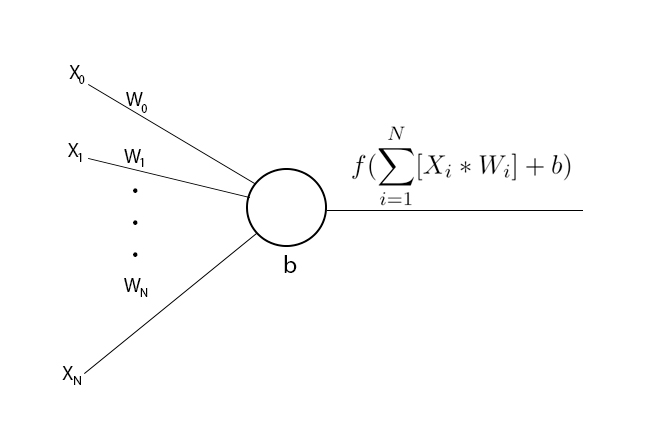
\includegraphics[scale=0.35]{imagenes/neurona.jpg}  
	\caption{Esquema de una neurona}
	\label{fig:neurona}
\end{figure}

Una neurona parte de una serie de datos de entrada X=\{$x_1$, $x_2$, ..., $x_N$\} tal que cada $x_i$$\in${X} se encuentra asociado a un peso $w_i\in{W}$ y obtiene un único dato de salida o resultado operando con los datos de entrada y sus pesos. \\
En la Figura \ref{fig:neurona} se muestra cómo esta los emplea para realizar una suma ponderada y posteriormente añadir un sesgo b, además de aplicar una función (que llamaremos función de activación) f sobre el resultado obtenido para obtener la salida. 

\subsection{Estructura por capas}

\begin{figure}[H]
	\centering
	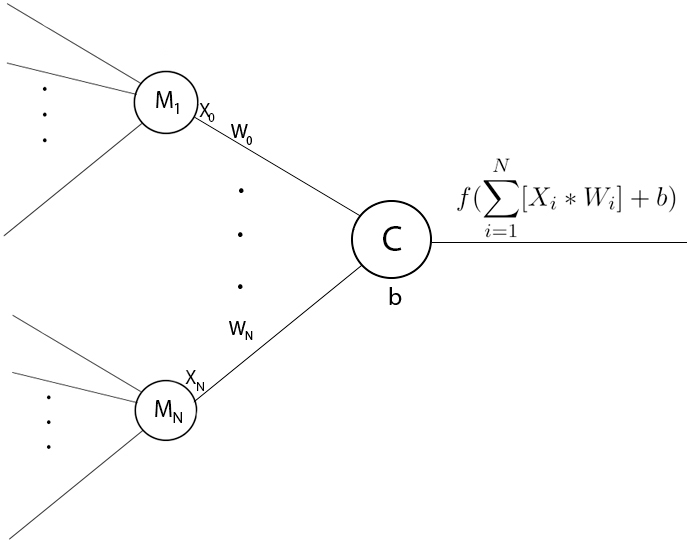
\includegraphics[scale=0.35]{imagenes/capa_neuronas.jpg}  
	\caption{Esquema de una capa de neuronas}
	\label{fig:capa_neuronas}
\end{figure}

Las neuronas se suelen agrupar por capas, de tal forma que la salida de una compone la entrada de la siguiente, formando así modelos más sofisticados. En la Figura \ref{fig:capa_neuronas}, se puede ver cómo la salida de la neurona C se obtiene tomando como entrada la salida de las neuronas $M_1, M_2, ..., M_N$.\\
En este proyecto se desarrollarán redes neuronales para tareas de clasificación multiclase. Para clasificar N clases distintas, la capa de salida tendrá N neuronas. De esta forma, nuestra red totalmente conectada tendrá una capa de entrada (para recibir los datos de entrenamiento), una capa de salida, y las capas intermedias entre estas dos recibirán el nombre de capas ocultas. 

\subsection{Funciones de activación}

Una función de activación, en el contexto de las redes neuronales, es una función matemática f que se aplica al resultado de sumar el producto escalar del vector de entrada y el vector de pesos con el sesgo para obtener la salida de una neurona. Su objetivo consiste en introducir no linealidad en el modelo, permitiendo que la red aprenda e identifique patrones complejos en los datos. Sin no linealidad, una red neuronal se comportaría esencialmente como un modelo de regresión lineal, independientemente del número de capas que tenga \cite{funcion_activacion_definicion}. Introduciremos a continuación una serie de funciones de activación de interés:

\subsubsection{Función ReLU}

\begin{gather}
	ReLU(x) = max(0, x)
\end{gather}

\begin{figure}[H]
	\centering
	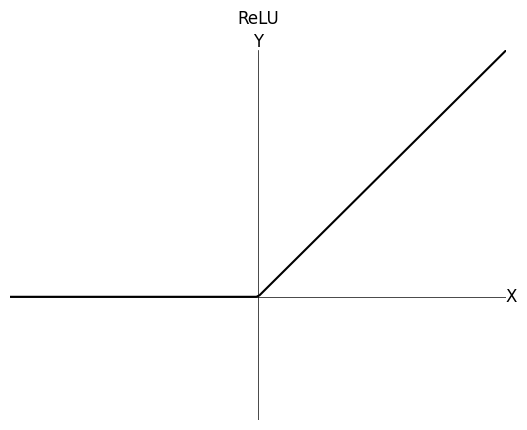
\includegraphics[scale=0.45]{imagenes/ReLU.jpg}  
	\caption{Imagen de la función de activación ReLU}
	\label{fig:ReLU}
\end{figure}

A cambio de un bajo coste computacional, la función de activación ReLU (véase la Figura \ref{fig:ReLU}) aporta no linealidad a la neurona, permitiendo a esta aprender funciones de mayor complejidad. \\
Como su gradiente es 0 ó 1 (0 para valores negativos, 1 para valores positivos), evita una reducción excesiva del mismo para valores positivos, mitigando así el problema del desvanecimiento del gradiente, caracterizado por la presencia de gradientes muy pequeños en retropropagación (se analizará esto con detalle en secciones posteriores) y provocar un aprendizaje lento \cite{ReLU}. \\
Además, tal y como sugieren los expertos, se empleará ReLU como función de activación en las capas intermedias de los modelos a implementar \cite{importancia_ReLU} \cite{importancia_ReLU_2}. 

\subsubsection{Función Sigmoide}

\begin{gather}
	sigmoide(x) = \frac{1}{1+e^{-x}}
\end{gather}

\begin{figure}[H]
	\centering
	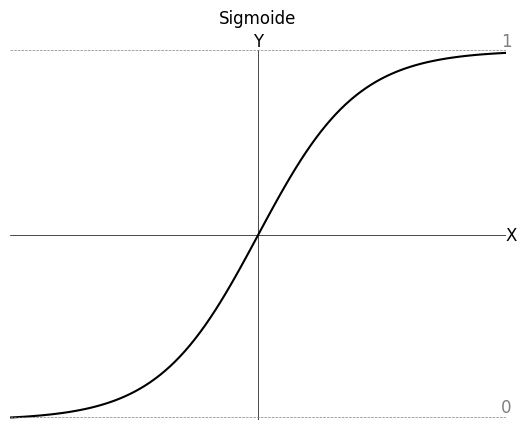
\includegraphics[scale=0.45]{imagenes/sigmoide.jpg}  
	\caption{Imagen de la función de activación Sigmoide}
	\label{fig:Sigmoide}
\end{figure}

Se define la función de activación Sigmoide como una función interesante en el ámbito de la clasificación binaria, pues es caracterizada por transformar un valor de entrada en una salida perteneciente al rango [0-1] , tal y como se muestra en la Figura \ref{fig:Sigmoide}. \\
Aunque sea monótona creciente y diferenciable en todos los puntos, tiende a saturarse con valores extremos (positivos o negativos). Por tanto, su aplicación dependerá del caso concreto a tratar. \cite{Sigmoide}

\subsection{Capa SoftMax}

\begin{figure}[H]
	\centering
	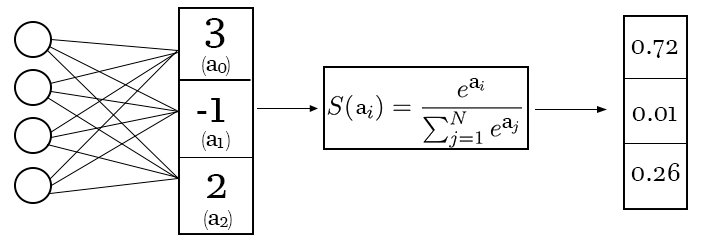
\includegraphics[scale=0.35]{imagenes/softmax.jpg}  
	\caption{Imagen de la función de activación SoftMax}
	\label{fig:SoftMax}
\end{figure}

La función SoftMax se suele emplear en la capa de salida de la red. Se caracteriza por, para N entradas, producir N salidas con valores en el rango [0-1] que mantienen la proporción de entrada y cuya suma es 1. Por tanto, cada salida i se puede interpretar como la probabilidad de pertenencia a la clase i, siendo especialmente útil en clasificación multiclase. \cite{SoftMax_MLM} \\
De esta forma, en la Figura \ref{fig:SoftMax} se muestra un ejemplo de clasificación multiclase con 3 clases distintas. \\
Para una entrada dada, el modelo estima que esta pertenece a la clase 0, pues según este, dicha entrada presenta un 72\% de probabilidad de pertenecer a la clase 0, un 1\% a la clase 1, y un 26\% a la clase 2.


\subsection{Tipos de codificaciones de etiquetas}

En el campo del machine learning existen varios tipos de codificaciones. Así, para codificar 3 clases distintas se podrían codificar o bien mediante \{1, 2, 3\}, o mediante \{100, 010, 001\} (codificación one-hot \cite{one_hot}), por ejemplo. En este proyecto se empleará la codificación one-hot por simplicidad y seguir el mismo enfoque seguido en la gran mayoría de bibliografía online.

\subsection{Función de error o pérdida}

En modelos de aprendizaje automático se suele emplear una función de optimización iterativa como descenso del gradiente (se muestra en el siguiente apartado) para, a partir de una función de error y unos datos de entrada, estimar el error del modelo sobre los mismos. Esta estimación del error se puede emplear para ir reduciendo el error iteración a iteración y así ir aprendiendo. 

\subsubsection{Entropía Cruzada}

\begin{gather}
	E(y, \hat{y}) = - \sum_{i=1}^{N}  [y_i log( \hat{y}_i)]
	\label{fig:loss_func_softmax}
\end{gather}

En los modelos a desarrollar en este proyecto, se empleará la Entropía Cruzada como función de error por ser una métrica empleada en aprendizaje automático para medir las prestaciones de un modelo de clasificación. La pérdida o error, se mide como un valor positivo mayor que 0, siendo 0 un modelo perfecto. \cite{Cross_entropy}

En la fórmula \ref{fig:loss_func_softmax}, se muestra la fórmula para el cálculo de la entropía cruzada, donde H es el número de clases al que puede pertenecer cada dato de entrada $x_i \in X$, $y_i$ representa la etiqueta real de la entrada $x_i$ empleada, e $\hat{y}_i$ representa la etiqueta que el modelo predijo para dicha entrada $x_i$.  \\

\subsection{Precisión}

\begin{gather}
	Precision = \frac{Predicciones\ correctas}{Predicciones\ totales}
	\label{accuracy_formula}
\end{gather}


En los modelos a desarrollar en este proyecto, se utilizará la precisión (accuracy) como métrica para evaluar la eficacia del modelo en la clasificación de un conjunto de datos específico. La precisión representa la proporción de predicciones correctas sobre el total de predicciones realizadas, y se calcula mediante la fórmula \ref{accuracy_formula}. Este valor se expresa como un porcentaje o como un número en el rango [0-1], donde 1 indica un modelo perfecto y 0 denota un modelo totalmente erróneo \cite{accuracy}. 

\subsubsection{Importancia de la función de error en el aprendizaje}

Para visualizar el papel de la función de error en el aprendizaje de un modelo, supondremos que los datos actuales cuentan con N=3 clases tal que, para un $x_i \in X$ dado y empleando la codificación One-Hot para las etiquetas, se tiene que $y_i = [0, 0, 1]$. 

\begin{gather}
	E(y, \hat{y}) = - \sum_{i=1}^{N}  [y_i log( \hat{y}_i)] = 0 + 0 + log(0.1) = -log(0.1) = 2.3
	\label{ejemplo_1}
\end{gather}

Como la configuración inicial del modelo es desconocida, se supone que sus predicciones iniciales para $x_i$ son $\hat{y_i} = [ 0.6, 0.3, 0.1]$. En este caso, $x_i$ pertenece a la clase 3 pero el modelo predice que pertenece a la clase 1, pues 0.6 se interpreta como la probabilidad de pertenecer a la clase 1 y es la probabilidad más grande de todo $\hat{y_i}$.\\
Por tanto, su función de error indicaría que el error obtenido viene dado por la fórmula \ref{ejemplo_1}.

\begin{gather}
	E(y, \hat{y}) = - \sum_{i=1}^{N}  [y_i log( \hat{y}_i)] = 0 + 0 + log(0.6) = -log(0.6) = 0.5
	\label{ejemplo_2}
\end{gather}

Tras entrenar el modelo durante varias iteraciones, $y_i$ permanece constante, pero $\hat{y_i}$ se modifica a $\hat{y_i} = [0.1, 0.3, 0.6]$, de forma que el nuevo error obtenido vendría dado por la fórmula \ref{ejemplo_2}, y ahora el modelo realizaría una predicción correcta sobre la clase de $x_i$, aunque todavía le quedaría margen de mejora pues el error es de 0.5 y este se puede minimizar. \\
De esta forma, se visualiza como, a lo largo del entrenamiento de un modelo, este se centra en reducir el error obtenido, y como consecuencia de ello va modificando sus predicciones, de tal forma que se vayan ajustando a lo especificado por sus datos de entrada y etiquetas asociadas.


% https://medium.com/mlearning-ai/understanding-loss-functions-for-classification-81c19ee72c2a

\subsection{Descenso del gradiente}

\begin{figure}[H]
	\centering
	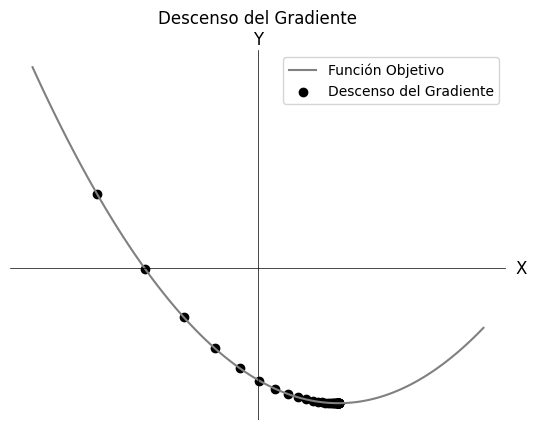
\includegraphics[scale=0.4]{imagenes/sgd.jpg}  
	\caption{Ejemplo de funcionamiento del descenso del gradiente}
	\label{fig:SGD}
\end{figure}

Tal y como se comentaba anteriormente, el descenso del gradiente es un método de optimización iterativo que busca el mínimo en una función diferenciable. En la figura \ref{fig:SGD} se muestra un ejemplo del mismo, donde la función objetivo a minimizar hace referencia a la función de pérdida, y cada punto sobre ella representa una iteración del algoritmo, indicando cómo el error del modelo sobre la muestra se va reduciendo con cada iteración. \\
Su nombre viene del término 'gradiente', siendo este una generalización multivariable de la derivada y denominado por el símbolo $\nabla$. Para una función f y un punto p, este indica la dirección del máximo incremento en la misma. El descenso del gradiente usa esta información para, una vez obtenido el gradiente, desplazarse en dirección contraria, es decir, en dirección del mínimo. Además, la distancia que se recorre en cada iteración viene dada por un hiperparámetro alpha denominado ``learning rate'' \cite{SGD_1} \cite{Gradiente} \cite{SGD_2}. \\
A diferencia de los parámetros de un modelo (pesos y sesgos), sus hiperparámetros son establecidos por el usuario y no se ``aprenden'' durante el entrenamiento del modelo.


\subsection{Inicialización de pesos}
Tal y como sugieren los expertos, se inicializarán los pesos mediante la ``inicialización He'' o ``inicialización Kaiming He''. Esta consiste en, para un peso $w$, inicializarlo según una distribución gaussiana con una media de 0.0 y una desviación típica de $\sqrt{\frac{2}{N\_in}}$, siendo $N\_in$ el número de neuronas en la capa de entrada
\cite{ini_He} \cite{ini_He_2} \cite{ini_He_code} \cite{importancia_ReLU} \cite{importancia_ReLU_2}.

\subsection{Inicialización de sesgos}

De la misma forma, se vuelve a seguir la bibliografía, indicando esta vez una inicialización de sesgos a 0.0 \cite{ini_bias} \cite{ini_bias_2}.

\subsubsection{Actualización de parámetros}
El procedimiento para entrenar una red neuronal consiste en, para una entrada $x_i$ y una etiqueta asociada $y_i$, emplear $x_i$ para realizar una predicción $\hat{y}_i$ (Propagación hacia delante de $x_i$ por la red) que posteriormente se podrá comparar con $y_i$ mediante una función de error H(x) y obtener una medida de lo buena o mala que fue la misma. Una vez obtenido dicho ``error'', se aplica el algoritmo del descenso del gradiente para obtener el gradiente de la pérdida respecto a cada parámetro de la red (Retropropagación) \cite{Cross_entropy}. \\

\begin{gather}
	W^{t+1}_i = W^{t}_i - \alpha \frac{\partial H(x)}{\partial W_{i}} 
	\label{act_pesos}
\end{gather}

\begin{gather}
	b_{t+1} = b_{t} - \alpha \frac{\partial H(x)}{\partial b_{t}}
	\label{act_bias}
\end{gather}


Así, se actualizarán los parámetros de la red neuronal (pesos y sesgos) según las fórmulas \ref{act_pesos} y \ref{act_bias}. En ellas, $W^t_i$ y $b_t$ indican los valores del peso $W_i$ y bias b en el instante o iteración t, de la misma forma que $W^{t+1}_i$ y $b_{t+1}$ representan los valores de los mismos en el instante t+1 \cite{SGD_act_params}. \\
Es decir, dada una iteración t y unos datos de entrada X, primero se realiza la propagación hacia delante de los mismos a lo largo del modelo para obtener  $\hat{Y}$ o la predicción de los mismos. Una vez obtenida $\hat{Y}$, se emplea la función de error para obtener el error del modelo sobre los datos de entrada. Con ello, se realiza la retropropagación del gradiente de la pérdida o error a lo largo del modelo, de forma que cada parámetro del mismo obtenga el gradiente de la pérdida respecto a él. Una vez cada parámetro tiene asociado su gradiente respecto a la pérdida, lo emplea junto con $\alpha$ para actualizar su valor, dirigiéndose en sentido contrario al gradiente con una magnitud igual a $\alpha$, permitiendo así la reducción del error en la iteración t+1. Los parámetros se actualizan una vez por iteración, tras realizar la retropropagación.

\subsubsection{Descenso del gradiente estocástico}

\begin{algorithm}[H]
	\caption{Descenso del gradiente estocástico \cite{SGD_3}} 
	\begin{algorithmic}
		\For{época $p\in\{0, ..., P-1\}$}
			\State Desordenar datos de entrenamiento.
			
			\For{$minibatch \in [m_{inicio}, ..., m_{fin}]$}
				\State Obtener datos del minibatch.
				\State Realizar propagación hacia delante.
				\State Obtener error mediante función de error.
				\State Realizar retropropagación y obtener gradiente de la pérdida   
				\State       respecto a cada parámetro del modelo.
				\State Actualizar parámetros.
			\EndFor
		\EndFor
	\end{algorithmic}
\end{algorithm}

El descenso del gradiente estocástico es una variante que sustituye el gradiente real por una estimación del mismo, logrando reducir la carga computacional y tiempo de entrenamiento a cambio de una menor tasa de convergencia \cite{sgd_stocastico} \cite{sgd_stocastico_1}. \\
Se caracteriza por, en cada época (un paso completo a través de todo el conjunto de datos de entrenamiento durante el proceso de aprendizaje \cite{sgd_stocastico}), dividir el conjunto de entrenamiento en varios subconjuntos aleatorios y disjuntos entre ellos (minibatch). \\
Para cada minibatch, se realiza la propagación hacia delante, el cálculo del error, la retropropagación y la actualización de parámetros en ese orden. \\


\subsection{Retropropagación en la capa SoftMax} 

Tal y como se comentó en secciones anteriores, se empleará SoftMax en la última capa totalmente conectada. De este modo, se definen los valores de entrada a la misma como \textit{Z}, y los de salida como \textit{O}, tal y como se muestra en la Figura \ref{cross_entropy_notacion}.

\begin{figure}[H]
	\centering
	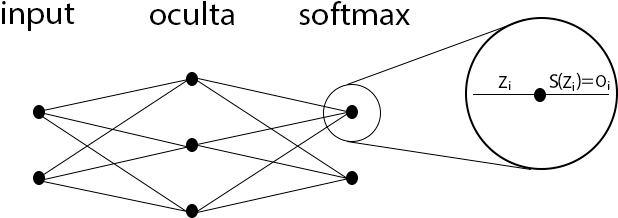
\includegraphics[scale=0.4]{imagenes/NN_softmax.jpg}  
	\caption{Estructura de una red totalmente conectada con una capa oculta, y con softmax en la última capa}
	\label{fig:nn_softmax_1_capa}
\end{figure}

Según esta notación, la función de error \ref{fig:loss_func_softmax} se convierte en la fórmula \ref{cross_entropy_notacion}.

\begin{gather}
	E = - \sum_{i=1}^{N}  [y_i ln(O_i)] 
	\label{cross_entropy_notacion}
\end{gather}

De este modo, se define el cálculo del gradiente de la pérdida, con respecto a cada neurona de entrada $Z_k$, de la capa SoftMax, según la fórmula \ref{gradiente_softmax} \cite{Cross_entropy_backprop} \cite{Cross_entropy_backprop_grad_input}. Para obtener una explicación detallada, y un desarrollo completo sobre los orígenes de dicha fórmula, consulte el apéndice \ref{softmax_apendice}.

\begin{gather}
	\frac{\partial E}{\partial Z_k} = O_k - y_k = gradiente\_Z_k
	\label{gradiente_softmax}
\end{gather}


\subsection{Retropropagación en redes neuronales rotalmente conectadas}

En esta sección, se analizará el cálculo del gradiente de la pérdida con respecto a cada parámetro entrenable de una red neuronal totalmente conectada, así como con respecto a la entrada y a la salida de cada capa. De este modo, se presentarán los cálculos aplicables a cualquier tipo de red totalmente conectada. Para obtener una explicación detallada, y un desarrollo completo sobre los orígenes de cada fórmula planteada en esta sección, se recomienda encarecidamente consultar el apéndice \ref{backprop_fully_apendice}.\\

Tal y como se muestra en la Figura \ref{fig:nn_softmax_1_capa}, se definen como capas ocultas todas aquellas capas situadas entre la capa de entrada y la capa de salida.
En particular, se definen como capas ocultas ``intermedias'' todas las capas, exceptuando la última de ellas, dado que estas capas comparten la mayoría de los cálculos asociados a la retropropagación. En consecuencia, una red neuronal totalmente conectada puede dividirse en 4 grupos $\{$capa de entrada, capas ocultas intermedias, última capa oculta, capa de salida o capa softmax$\}$. \\
A continuación, se realiza el cálculo necesario para la retropropagación de una capa de neuronas \textit{l} específica. Suponemos que la capa \textit{l+1} tiene \textit{Q} neuronas, la capa \textit{l-1} tiene \textit{K} neuronas, y que todas las capas ocultas intermedias usan ReLU como función de activación. \\

\subsubsection{Gradiente respecto a la entrada de la capa}

\begin{figure}[H]
	\centering
	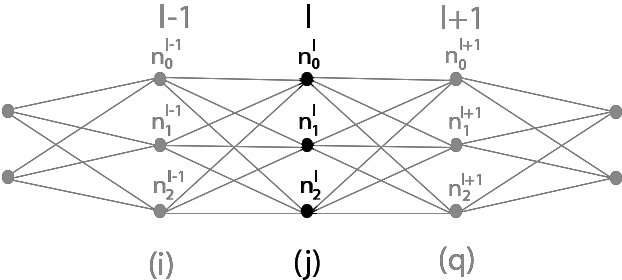
\includegraphics[scale=0.35]{imagenes/conclusion_capa_l.jpg}  
	\caption{Retropropagación en la capa l}
	\label{fig:conclusion_capa_l}
\end{figure}

La Figura \ref{fig:conclusion_capa_l} muestra una representación en la que los 'puntos' están interconectados mediante líneas, los cuales representan neuronas artificiales, y los pesos que las conectan, respectivamente. Cada punto corresponde a una neurona, y, cada línea, a un peso. El superíndice indica la capa a la que pertenece una neurona o peso, mientras que el subíndice especifica el número de la neurona o peso en su respectiva capa. En el caso de los pesos, se requieren 2 subíndices para identificar a cada uno, ya que cada peso conecta 2 neuronas. \\
En este contexto, la capa oculta l está compuesta por 3 neuronas, denotadas como $n^{l}_0$, $n^{l}_1$, y $n^{l}_2$. De este modo. se define como $W^{i}_{jq}$ al peso que une las neuronas $n^{i}_j$ y $n^{i+1}_q$. 
Para la neurona $n^l_j$, se denota como $a^l_j$ el valor de la neurona antes de aplicar la función de activación asociada, y como $z^l_j$, el valor obtenido después de aplicar dicha función. 
Además, se define como $gradiente\_a_{{l+1}_q}$ al gradiente de la pérdida con respecto a $a^{l+1}_q$. Asimismo, se denota como $ReLU'(a^l_j)$ a la derivada de la función de activación ReLU aplicada al valor $(a^l_j)$.\\

\begin{gather}
	\frac{\partial E_{total}}{\partial a^l_j} = \sum_{q=1}^Q  gradiente\_a_{{l+1}_q} W^l_{ij} ReLU'(a^l_j) \label{grad_input_l_4}
\end{gather}

La fórmula \ref{grad_input_l_4}, ilustra el cálculo necesario para determinar el gradiente de la función de pérdida, con respecto a la neurona de entrada j, de una capa oculta intermedia \textit{l}, $\frac{\partial E_{total}}{\partial a^l_j}$, a partir del gradiente de la función de pérdida, con respecto a la entrada de capa \textit{l+1}, $gradiente\_a_{{l+1}_q}$.


\subsubsection{Gradiente respecto a los pesos}

\begin{figure}[H]
	\centering
	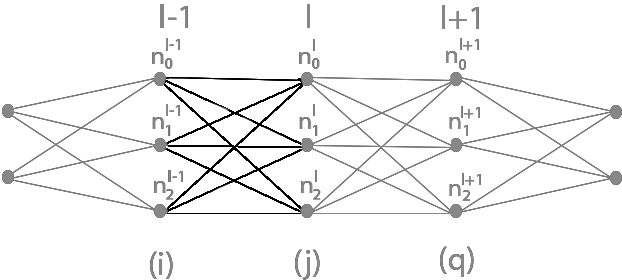
\includegraphics[scale=0.35]{imagenes/conclusion_pesos.jpg}  
	\caption{Retropropagación respecto a los pesos entre la capa l-1 y l}
	\label{fig:conclusion_pesos}
\end{figure}

\begin{gather}
	\frac{\partial E_{total} }{\partial W^{l-1}_{ij} } = gradiente\_h_{l_j} z^{l-1}_i \label{grad_w_l_3}
\end{gather}

La fórmula \ref{grad_w_l_3}, detalla el cálculo necesario para determinar el gradiente de la pérdida, con respecto a los pesos entre las capas ocultas \textit{l} y \textit{l-1}.

\subsection{Gradiente respecto a sesgos}

\begin{gather}
	\frac{\partial E}{\partial b^l_j} = gradiente\_h_{l_j} \label{grad_b_l_3}
\end{gather}

La fórmula \ref{grad_b_l_3} muestra el cálculo necesario para determinar el gradiente de la función de pérdida con respecto a los sesgos de la capa oculta \textit{l}.



\section{Redes Neuronales Convolucionales}

Las redes neuronales convolucionales \cite{CNN_definicion} surgen como una adaptación de las redes neuronales totalmente conectadas para el caso concreto de tratamiento de imágenes. Ambas comparten la idea de contar con una serie de neuronas artificiales distribuidas por capas de forma de la salida de la capa i sea la entrada de la capa i+1. Su principal diferencia reside en los datos de entrada y en las operaciones que se realizan en cada capa. Por ello, en secciones posteriores, se introducirán en detalle dos nuevas capas (capa convolucional y capa de agrupación máxima), cada una caracterizada por realizar un tipo de operación distinto.

\subsection{Introducción a CNNs \label{intro_CNN}}

\begin{figure}[H]
	\hspace{-10mm}
	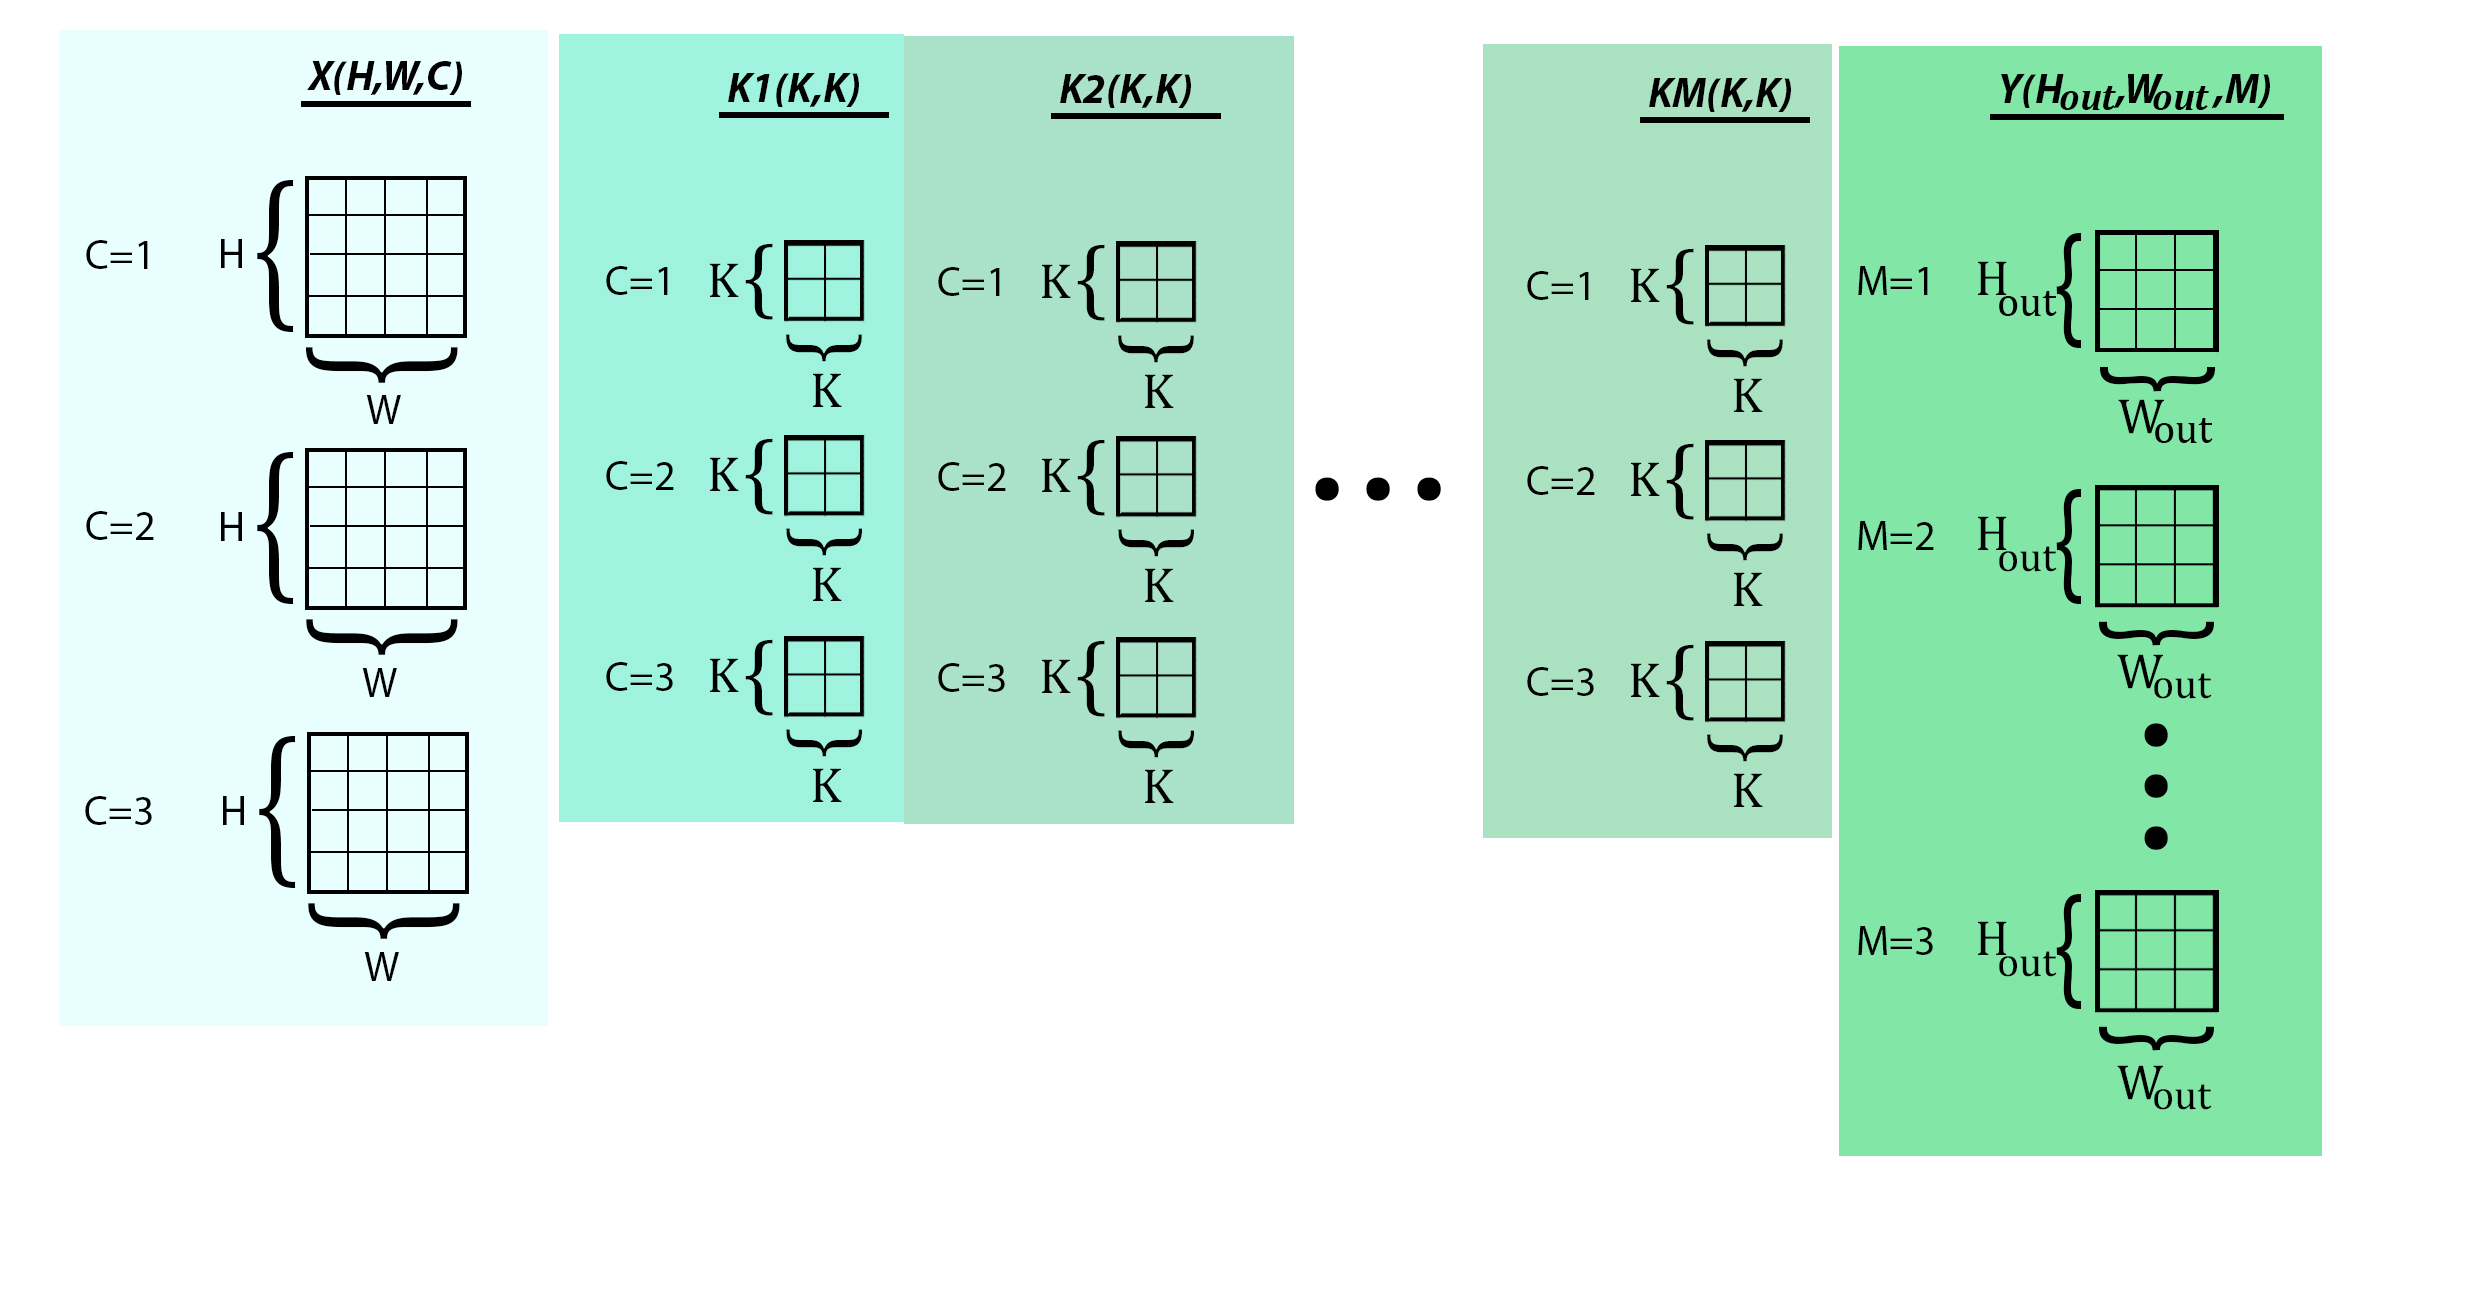
\includegraphics[scale=0.2]{imagenes/conv_dims.jpg}  
	\caption{Esquema de las dimensiones en una capa convolucional de una red neuronal convolucional}
	\label{fig:Dimensiones_convolucion}
\end{figure}


Las redes neuronales convolucionales (CNN, Convolutional Neural Network) se distinguen por su capacidad para trabajar con volúmenes de datos 3D. En este proyecto, se emplearán imágenes RGB como entrada para cada CNN. De este modo, cada imagen RGB puede interpretarse como un conjunto de capas 2D. De esta manera, si definimos X como un volumen 3D que representa una imagen RGB, X estará compuesto por 3 imágenes 2D, cada una correspondiente a un color (rojo, verde y azul). 
Adicionalmente, las dimensiones de X se definen como H (filas), W (columnas) y C(canales de profundidad), o, de forma abreviada, X(H,W,C) (véase la Figura \ref{fig:Dimensiones_convolucion}). \\
De manera equivalente, en una capa convolucional, los kernels de pesos se definen como $\{K_1, K_2, ..., K_M\}$ o $\{K_1(K,K), K_2(K,K), ..., K_M(K,K)\}$, donde cada uno de ellos tendrá K filas y K columnas. \\
Finalmente, en cada capa de una red neuronal convolucional, se define el volumen de salida como Y o Y($H_{out}, W_{out}, M$), y estará compuesto de $H_{out}$ filas, $W_{out}$ columnas, y M canales de profundidad, (uno por kernel de pesos).

\subsection{Estructura por capas}

\begin{figure}[H]
	\centering
	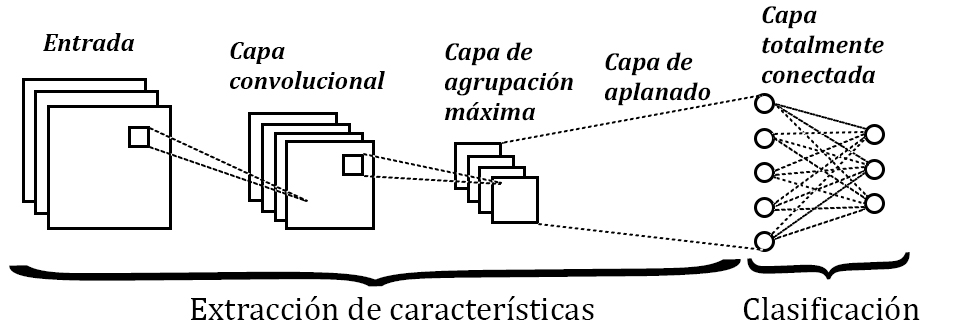
\includegraphics[scale=0.35]{imagenes/CNN_estructura.jpg}  
	\caption{Estructura por capas en una red neuronal convolucional}
	\label{fig:CNN_estructura}
\end{figure}

La arquitectura básica de una CNN se compone de dos partes principales (véase la Figura \ref{fig:CNN_estructura}):

\begin{enumerate} [label=\textbullet]
	\item \textbf{Extracción de Características}: Se define como extracción de características, al proceso que emplea múltiples pares de capas convolucionales y de agrupamiento máxima. Estas, se emplean para reducir y resumir las características de especial importancia, presentes en el conjunto de datos original.
	\item \textbf{Clasificación}: Una vez obtenido el resultado del proceso de extracción de características, en la etapa de clasificación, se emplea para predecir la clase de las imágenes de entrada. La capa totalmente conectada, realiza la clasificación final, combinando la información procesada en las etapas anteriores.
\end{enumerate}

A continuación, se define cada una de las capas involucradas en una red neuronal convolucional:

\begin{enumerate}[label=\textbullet]
	\item \textbf{Capa convolucional}: La capa convolucional, extrae características de la entrada X mediante la operación de convolución, y esta se realiza con un filtro de tamaño KxK. De esta manera, genera un mapa de características de salida (Y), que preserva la relación espacial entre los píxeles, y resalta elementos clave como bordes y esquinas.
	\item \textbf{Capa de agrupación máxima}: Se define como capa de agrupación máxima, aquella centrada en reducir la dimensionalidad de la entrada. Dicha reducción se obtiene al seleccionar, dentro de una región definida de la entrada, el valor máximo, preservando así las características más relevantes. Esta operación no solo disminuye la complejidad computacional, sino que también contribuye a que la red sea más invariante a pequeñas traslaciones en la entrada.
	\item \textbf{Capa de aplanado}: Se define como capa de aplanado aquella que transforma un volumen tridimensional en un vector unidimensional. De este modo, facilita la transición de las características extraídas por capas convolucionales y de agrupamiento hacia capas totalmente conectadas.
	\item \textbf{Capa totalmente conectada}: Se define como capa totalmente conectada aquella en la que cada neurona está conectada a todas las neuronas de la capa anterior y posterior. De este modo, permite la combinación de todas las características extraídas para realizar la clasificación multiclase que se llevará a cabo en este proyecto.
\end{enumerate}

\subsection{Capa convolucional}

\subsubsection{Componentes}


\begin{figure}[H]
	\centering
	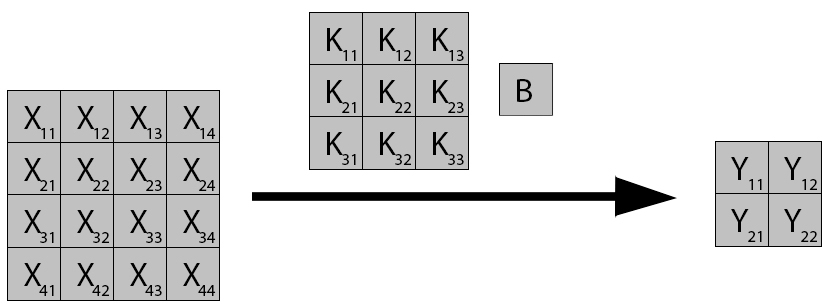
\includegraphics[scale=0.35]{imagenes/conv_nombres.jpg}  
	\caption{Componentes en una capa convolucional}
	\label{fig:Componentes_convolucion}
\end{figure}

Una capa convolucional parte de un volumen de entrada X, un kernel de filtros K, un sesgo B y una función de activación para, mediante una convolución, obtener un volumen de salida Y \cite{capa_convolucional} \cite{capa_convolucional_Stanford}.

\subsubsection{Propagación hacia delante}

\begin{figure}[H]
	\centering
	\begin{subfigure}{.5\textwidth}
		\hspace{-10mm}
		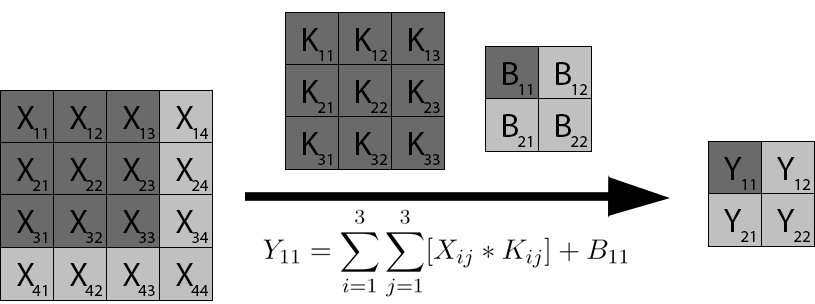
\includegraphics[width=1.2\linewidth]{imagenes/conv_1.jpg}  
		\caption{Cálculo $Y_{11}$}
	\end{subfigure}%
	\begin{subfigure}{.5\textwidth}
		\hspace{10mm}
		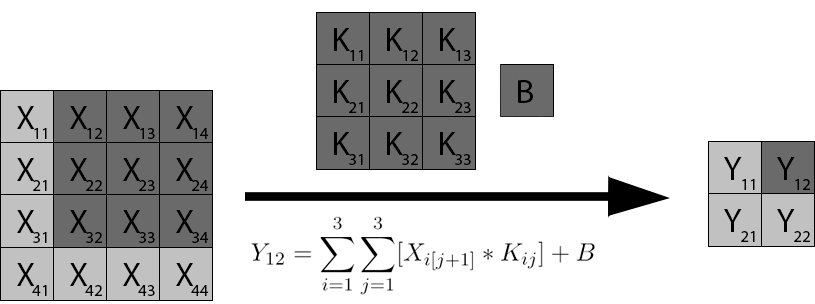
\includegraphics[width=1.2\linewidth]{imagenes/conv_2.jpg}  
		\caption{Cálculo $Y_{12}$}
	\end{subfigure}
	
	\vspace{5mm}
	\begin{subfigure}{.5\textwidth}
		\hspace{-10mm}
		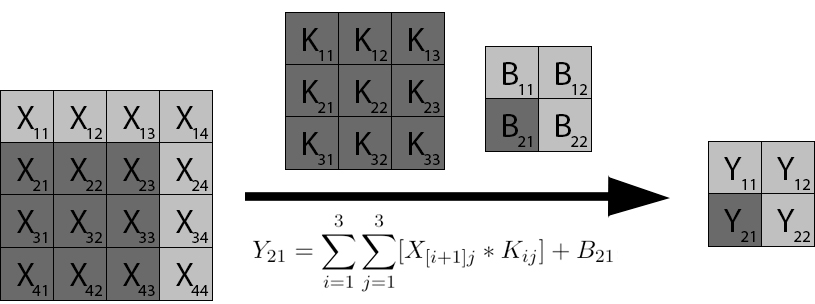
\includegraphics[width=1.2\linewidth]{imagenes/conv_3.jpg}  
		\caption{Cálculo $Y_{21}$}
	\end{subfigure}%
	\begin{subfigure}{.5\textwidth}
		\hspace{10mm}
		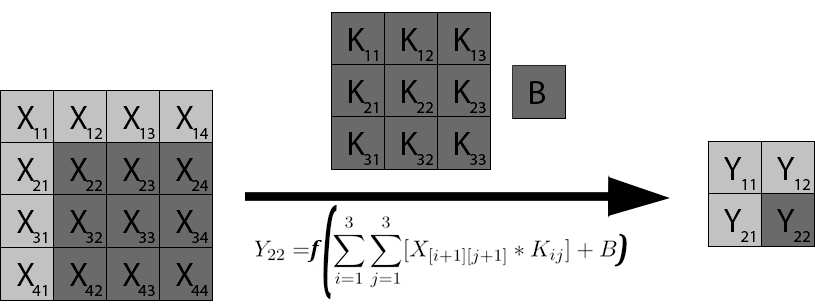
\includegraphics[width=1.2\linewidth]{imagenes/conv_4.jpg}  
		\caption{Cálculo $Y_{22}$}
	\end{subfigure}
	\caption{Propagación hacia delante en una capa convolucional}
	\label{fig:forward_prop_convolucional}
\end{figure}

Una convolución entre 2 volúmenes de datos X y K, consiste en ``deslizar K sobre X'' tal y como se muestra en la Figura \ref{fig:forward_prop_convolucional}. 
De esta forma, en cada ``paso'' se recorren ambos volúmenes, multiplicando los elementos de X y K que se encuentren superpuestos en la misma posición. Posteriormente, se suma cada resultado obtenido, además de un sesgo B y finalmente se aplica una función de activación \cite{capa_convolucional}. \\
Por simplicidad inicial, en la Figura \ref{fig:forward_prop_convolucional} se emplea un volumen X con un solo canal de profundidad. Sin embargo, este no es el caso común. Por tanto, se denotará como $X^{c}_{ij}$ al elemento de X que se encuentre en la posición (i,j) del canal de profundidad c. De la misma forma, se definirá $K^{c}_{ij}$ como el peso $k \in K$ que se encuentre en la posición (i, j) del canal de profundidad c del kernel de pesos K \cite{capa_convolucional_Stanford}.

\subsubsection{Propagación hacia delante de X con varios canales de profundidad}

\begin{figure}[H]
	\centering
	\begin{subfigure}{.5\textwidth}
		\hspace{-10mm}
		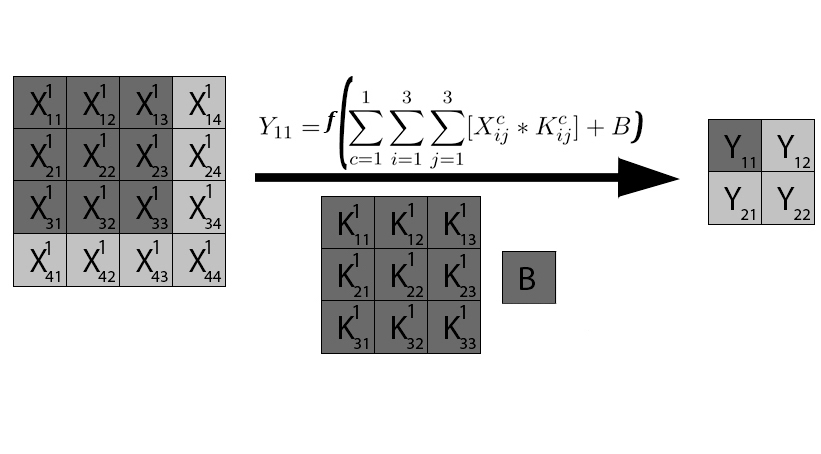
\includegraphics[width=1.2\linewidth]{imagenes/conv_1_1canal.jpg}  
		\caption{Cálculo $Y_{11}$ con entrada X \\ de 1 canal de profundidad}
	\end{subfigure}%
	\begin{subfigure}{.5\textwidth}
		\hspace{10mm}
		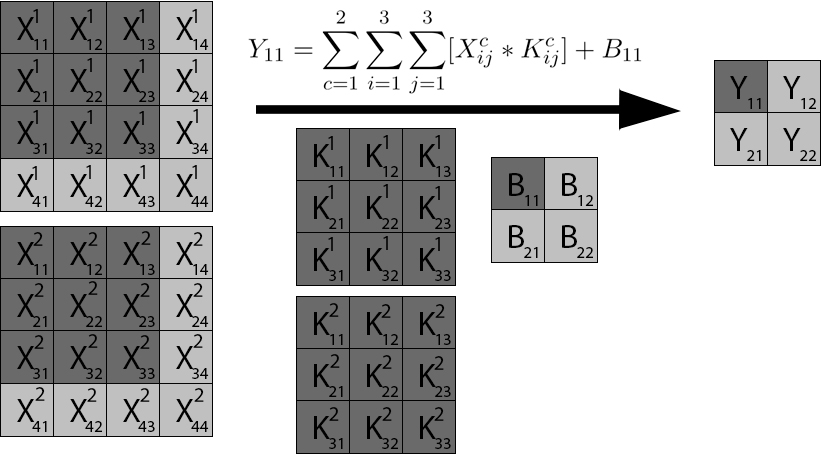
\includegraphics[width=1.2\linewidth]{imagenes/conv_1_2canales.jpg}  
		\caption{Cálculo $Y_{11}$ con entrada X \\ de 2 canales de profundidad}
	\end{subfigure}
	
	\vspace{5mm}
	\begin{subfigure}{.5\textwidth}
		\hspace{-10mm}
		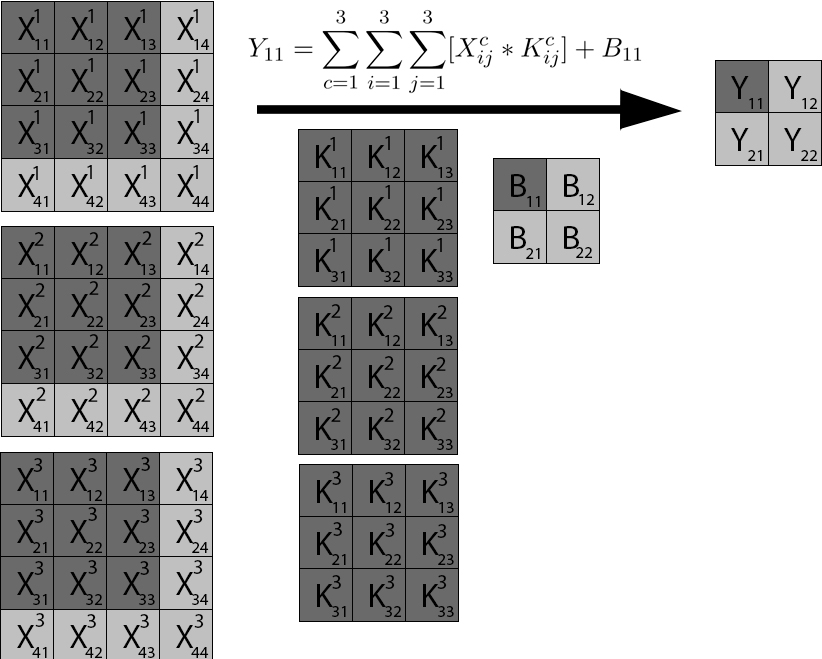
\includegraphics[width=1.2\linewidth]{imagenes/conv_1_3canales.jpg}  
		\caption{Cálculo $Y_{11}$ con entrada X \\ de 3 canales de profundidad}
	\end{subfigure}
	\caption{Propagación hacia delante en una capa convolucional con varios canales de profundidad}
	\label{fig:forward_prop_convolucional_canales_profundidad}
\end{figure}

De esta forma, en la Figura \ref{fig:forward_prop_convolucional_canales_profundidad} se muestra como una convolución con C canales de profundidad se descompone en la suma de C convoluciones con un canal de profundidad (véase la fórmula \ref{descomposicion_convoluciones_C_canales}).  \\
Por último, en cada ``paso'' del ``deslizamiento'' se suma un solo sesgo y se aplica una sola vez la función de activación, independientemente del número de canales de profundidad que presente la entrada X.

\begin{equation}
	\begin{split}
		\text{convolucion\_C\_canales}(X,K) = \text{convolucion\_1\_canal}(X^1,K^1) + \\
		\text{convolucion\_1\_canal}(X^2,K^2) + \cdots + \text{convolucion\_1\_canal}(X^C,K^C)
	\end{split}
	\label{descomposicion_convoluciones_C_canales}
\end{equation}


\subsubsection{Propagación hacia delante de X con varios filtros}

\begin{figure}[H]
	\centering
	\begin{subfigure}{.5\textwidth}
		\hspace{-10mm}
		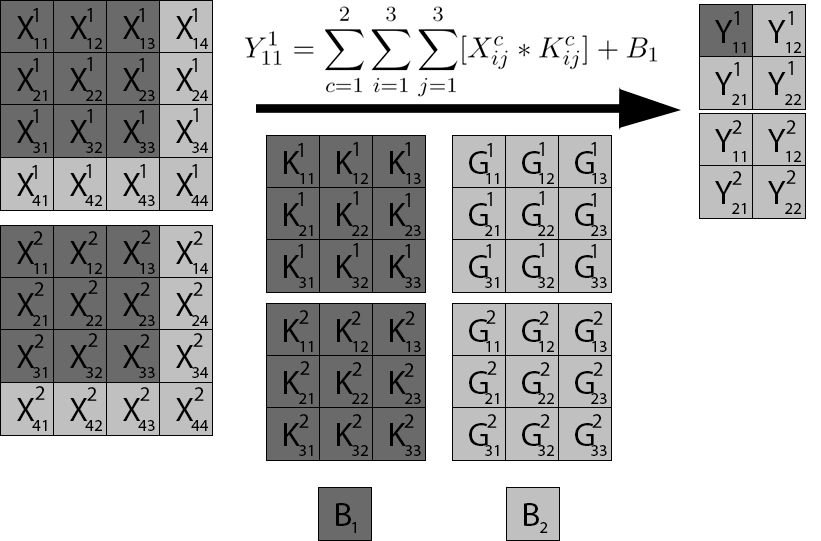
\includegraphics[width=1.2\linewidth]{imagenes/conv_2kernels_1.jpg}  
		\caption{Cálculo de $Y^1_{11}$ con el filtro K}
	\end{subfigure}%
	\begin{subfigure}{.5\textwidth}
		\hspace{10mm}
		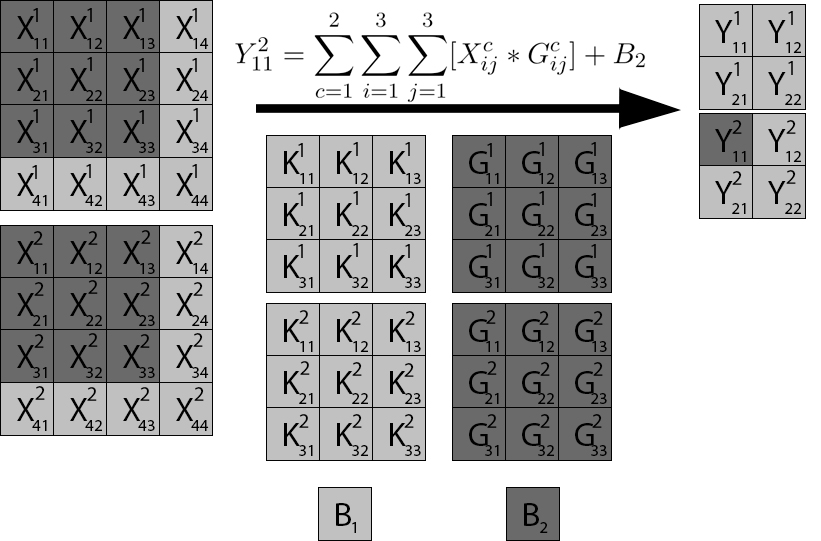
\includegraphics[width=1.2\linewidth]{imagenes/conv_2kernels_2.jpg}  
		\caption{Cálculo $Y^2_{11}$ con el filtro G}
	\end{subfigure}
	\caption{Propagación hacia delante en una capa convolucional con varios filtros}
	\label{fig:forward_prop_convolucional_varios_kernels}
\end{figure}

Cada convolución entre dos volúmenes 3D produce un volumen de salida 2D. Por tanto, al aplicar M convoluciones entre un volumen de entrada X y una serie de filtros K=$\{K_1, K_2, ..., K_M\}$, se obtendrá un volumen 3D de salida con tantas capas de profundidad como convoluciones se aplicaron (M). \\
En la Figura \ref{fig:forward_prop_convolucional_varios_kernels} se observa como al aplicar M=2 convoluciones sobre la misma entrada X (una con el filtro K y otra con el filtro G) se obtiene un volumen de salida con 2 capas de profundidad \cite{capa_convolucional_Stanford}.

\subsubsection{Relleno o ``Padding''}

En la figura \ref{fig:forward_prop_convolucional} se visualiza como al realizar una convolución entre un volumen X con dimensiones 1x4x4 y un kernel de pesos K con dimensiones 1x3x3, el resultado obtenido es un volumen Y de dimensiones 1x2x2. La reducción de dimensionalidad es un problema pues afecta directamente al número de convoluciones que se pueden aplicar sobre un volumen. \\
Por tanto, el ``relleno' o ``padding'' \cite{padding_definicion} se aplica antes de realizar una convolución y es una técnica empleada para conservar las dimensiones espaciales de un volumen de entrada X, expandiendo cada canal del mismo tal y como se muestra en la figura \ref{fig:padding} \cite{padding_1}.

\begin{figure}[H]
	\centering
	\begin{subfigure}{.5\textwidth}
		\hspace{-15mm}
		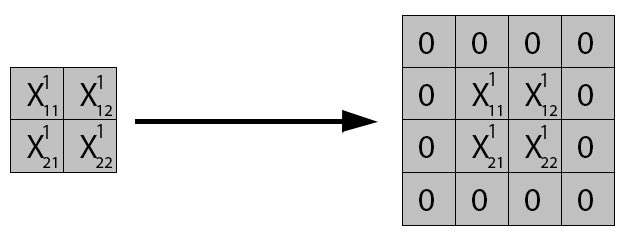
\includegraphics[width=1.2\linewidth]{imagenes/padding_a_1_nivel.jpg}  
		\caption{1 nivel de relleno}
	\end{subfigure}%
	\begin{subfigure}{.5\textwidth}
		\hspace{5mm}
		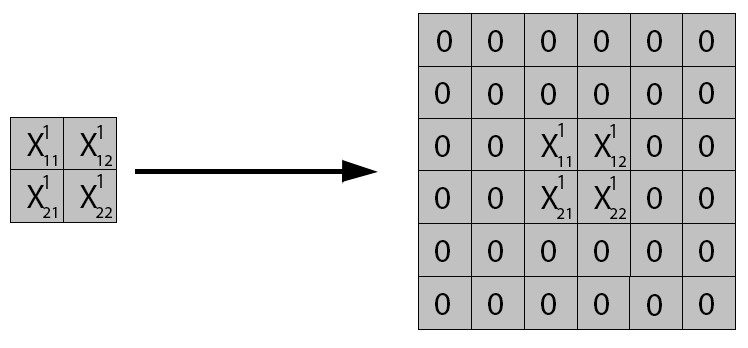
\includegraphics[width=1.2\linewidth]{imagenes/padding_a_2_niveles.jpg}  
		\caption{2 niveles de relleno}
	\end{subfigure}
	\caption{Relleno sobre un volumen de entrada X}
	\label{fig:padding}
\end{figure}

De esta forma, un relleno a un nivel sobre un volumen añadirá sobre el mismo dos filas y dos columnas con valores igual a 0. Un relleno a dos niveles añadirá cuatro filas y columnas con valores igual a cero, ..., un relleno a n niveles añadirá 2n filas y columnas con valores igual a 0.

\subsubsection{Relleno completo}

Se denomina como relleno completo \cite{full_padding_definicion} \cite{padding_2} aquel que asegura que cada valor o casilla de X sea visitada el mismo número de veces que el resto en una operación de convolución.

\begin{figure}[H]
	\centering
	\subfloat[visitas$\{x_{11}$:1, $x_{12}$:0, $x_{21}$:0, $x_{22}$: 0$\}$]{%
		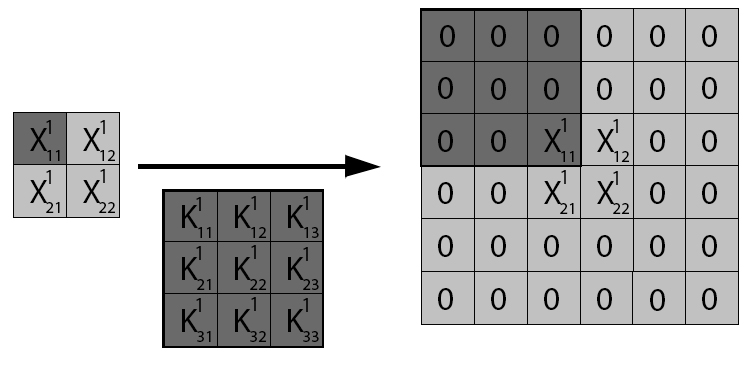
\includegraphics[width=0.45\textwidth]{imagenes/conv_padding_1.jpg}%
		\label{fig:sub1}%
	}\hfill
	\subfloat[visitas$\{x_{11}$:2, $x_{12}$:1, $x_{21}$:0, $x_{22}$: 0$\}$]{%
		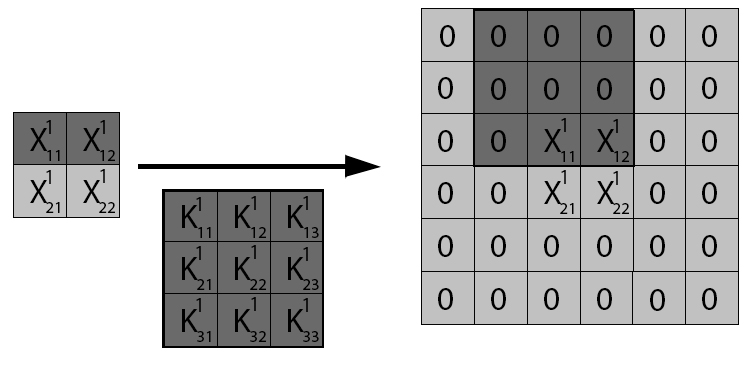
\includegraphics[width=0.45\textwidth]{imagenes/conv_padding_2.jpg}%
		\label{fig:sub2}%
	}\\
	\subfloat[visitas$\{x_{11}$:3, $x_{12}$:2, $x_{21}$:0, $x_{22}$: 0$\}$]{%
		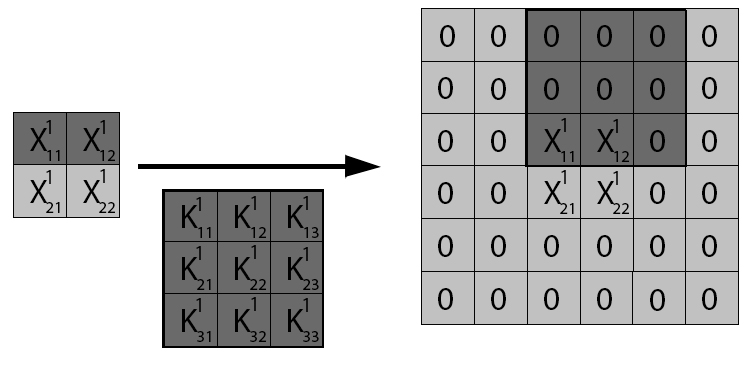
\includegraphics[width=0.45\textwidth]{imagenes/conv_padding_3.jpg}%
		\label{fig:sub3}%
	}\hfill
	\subfloat[visitas$\{x_{11}$:3, $x_{12}$:3, $x_{21}$:0, $x_{22}$: 0$\}$]{%
		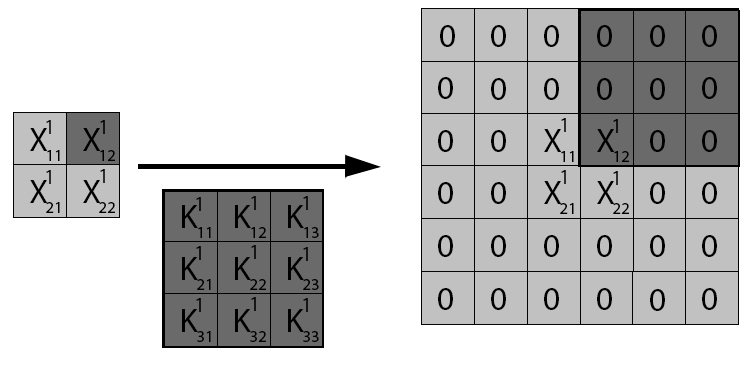
\includegraphics[width=0.45\textwidth]{imagenes/conv_padding_4.jpg}%
		\label{fig:sub4}%
	}\hfill
	
	\caption{Relleno sobre un volumen de entrada X}
\end{figure}

\begin{figure}[H]\ContinuedFloat
	\centering
	\subfloat[visitas$\{x_{11}$:4, $x_{12}$:3, $x_{21}$:1, $x_{22}$: 0$\}$]{%
		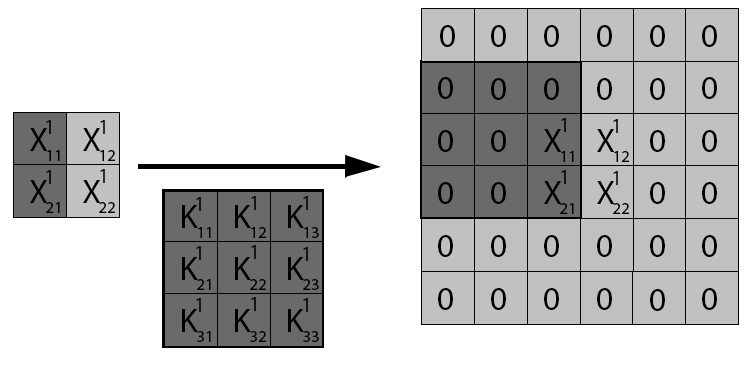
\includegraphics[width=0.45\textwidth]{imagenes/conv_padding_5.jpg}%
		\label{fig:sub5}%
	}\hfill
	\subfloat[visitas$\{x_{11}$:5, $x_{12}$:4, $x_{21}$:2, $x_{22}$: 1$\}$]{%
		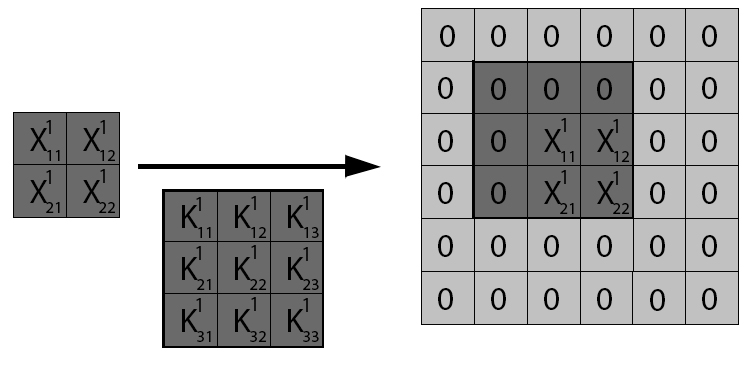
\includegraphics[width=0.45\textwidth]{imagenes/conv_padding_6.jpg}%
		\label{fig:sub6}%
	}\\
	\subfloat[visitas$\{x_{11}$:6, $x_{12}$:5, $x_{21}$:3, $x_{22}$: 2$\}$]{%
		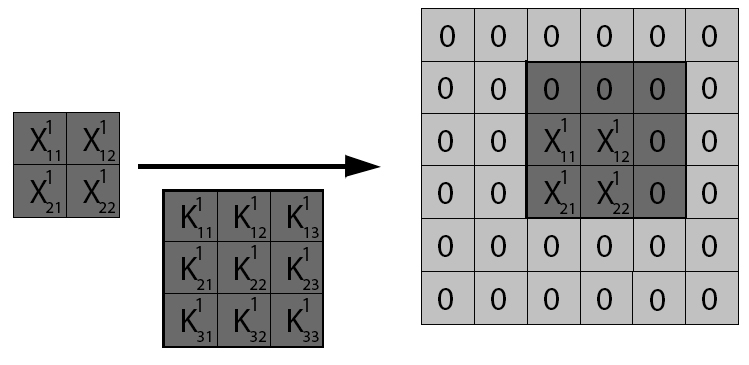
\includegraphics[width=0.45\textwidth]{imagenes/conv_padding_7.jpg}%
		\label{fig:sub7}%
	}\hfill
	\subfloat[visitas$\{x_{11}$:6, $x_{12}$:6, $x_{21}$:3, $x_{22}$: 3$\}$]{%
		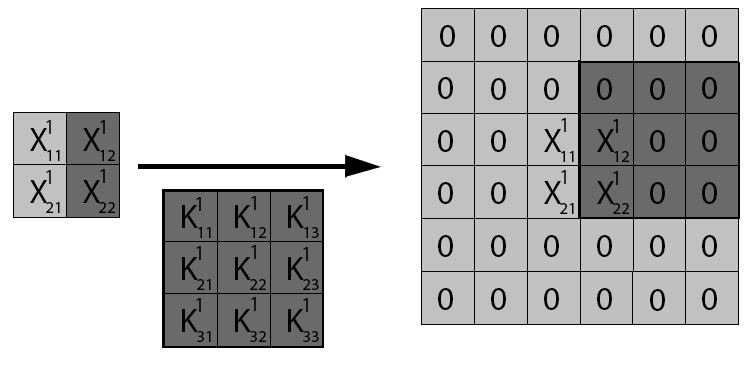
\includegraphics[width=0.45\textwidth]{imagenes/conv_padding_8.jpg}%
		\label{fig:sub8}%
	}\hfill
		\subfloat[visitas$\{x_{11}$:7, $x_{12}$:6, $x_{21}$:4, $x_{22}$: 3$\}$]{%
		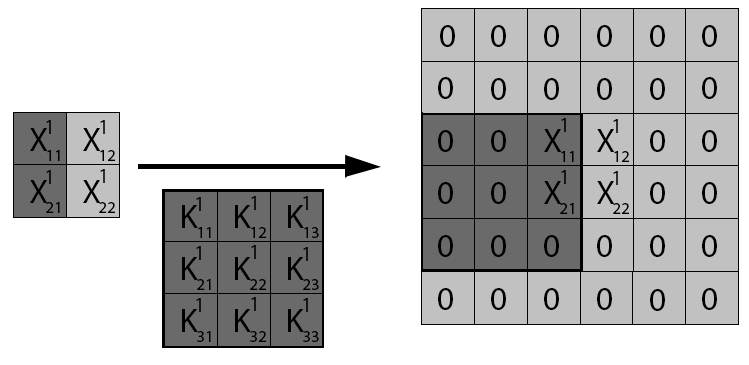
\includegraphics[width=0.45\textwidth]{imagenes/conv_padding_9.jpg}%
		\label{fig:sub9}%
	}\hfill
	\subfloat[visitas$\{x_{11}$:8, $x_{12}$:7, $x_{21}$:5, $x_{22}$: 4$\}$]{%
		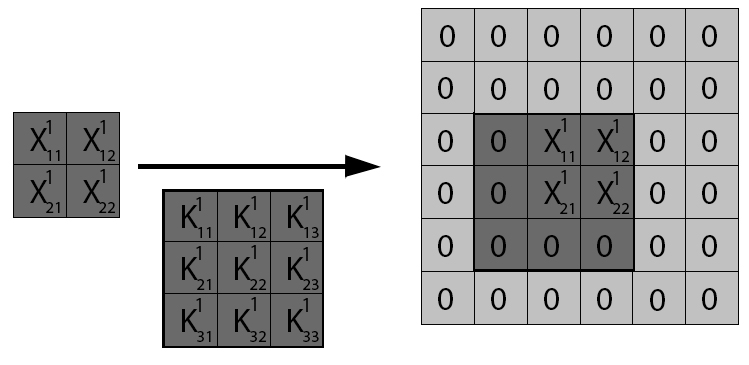
\includegraphics[width=0.45\textwidth]{imagenes/conv_padding_10.jpg}%
		\label{fig:sub10}%
	}\hfill
		\subfloat[visitas$\{x_{11}$:9, $x_{12}$:8, $x_{21}$:6, $x_{22}$: 5$\}$]{%
		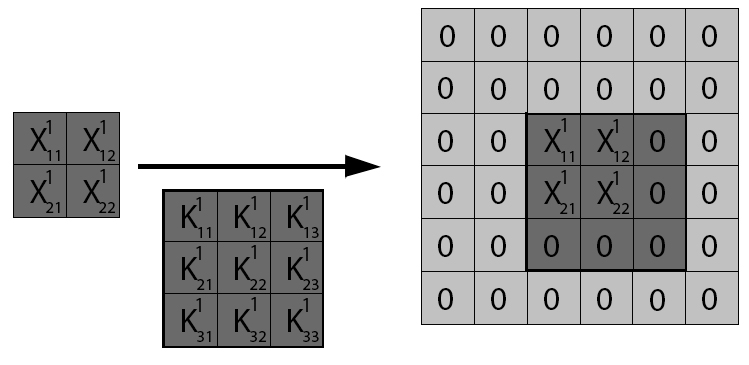
\includegraphics[width=0.45\textwidth]{imagenes/conv_padding_11.jpg}%
		\label{fig:sub11}%
	}\hfill
	\subfloat[visitas$\{x_{11}$:9, $x_{12}$:9, $x_{21}$:6, $x_{22}$: 6$\}$]{%
		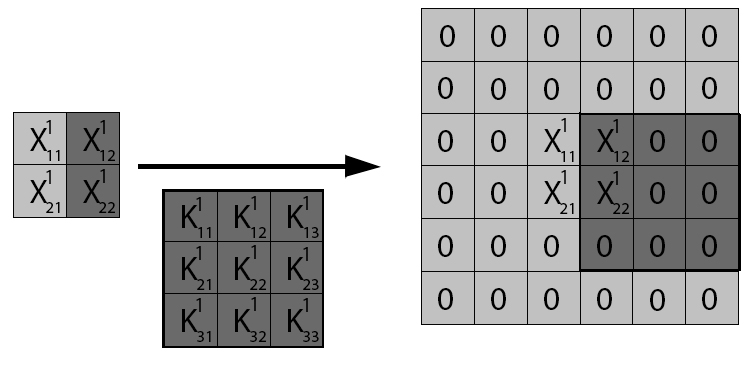
\includegraphics[width=0.45\textwidth]{imagenes/conv_padding_12.jpg}%
		\label{fig:sub12}%
	}\hfill
	\subfloat[visitas$\{x_{11}$:9, $x_{12}$:9, $x_{21}$:7, $x_{22}$: 6$\}$]{%
		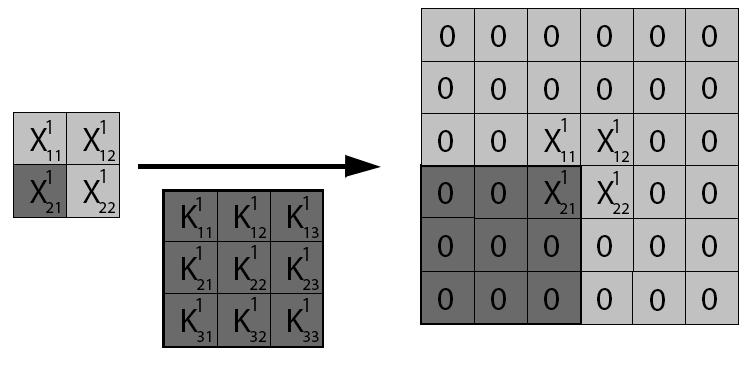
\includegraphics[width=0.45\textwidth]{imagenes/conv_padding_13.jpg}%
		\label{fig:sub13}%
	}\hfill
	\subfloat[visitas$\{x_{11}$:9, $x_{12}$:9, $x_{21}$:8, $x_{22}$: 7$\}$]{%
		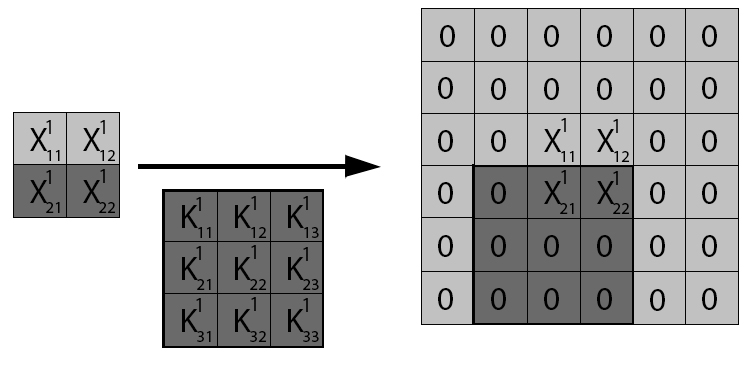
\includegraphics[width=0.45\textwidth]{imagenes/conv_padding_14.jpg}%
		\label{fig:sub14}%
	}\hfill
	\subfloat[visitas$\{x_{11}$:9, $x_{12}$:9, $x_{21}$:9, $x_{22}$: 8$\}$]{%
		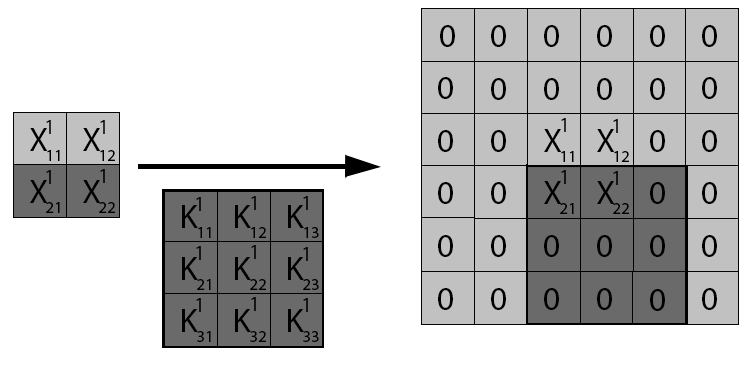
\includegraphics[width=0.45\textwidth]{imagenes/conv_padding_15.jpg}%
		\label{fig:sub15}%
	}\hfill
	\subfloat[visitas$\{x_{11}$:9, $x_{12}$:9, $x_{21}$:9, $x_{22}$: 9$\}$]{%
		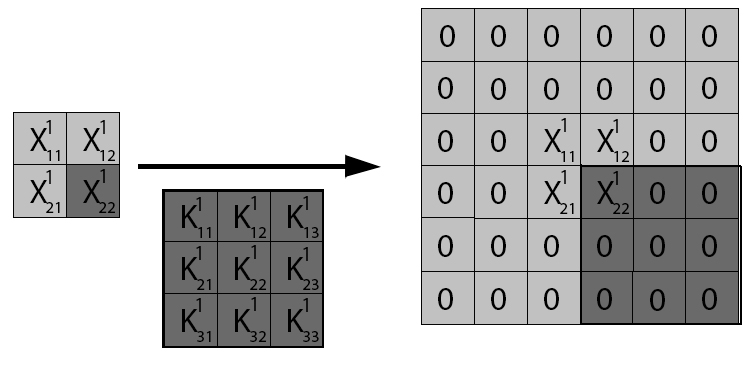
\includegraphics[width=0.45\textwidth]{imagenes/conv_padding_16.jpg}%
		\label{fig:sub16}%
	}\\
	
	\caption{Convolución sobre X con relleno completo}
	\label{fig:full_padding}
\end{figure}

Tal y como se muestra en la figura \ref{fig:full_padding}, se realiza un relleno completo pues en la convolución entre X y K se accede a cada valor de X el mismo número de veces (9).


\subsection{Retropropagación en capas convolucionales}

\begin{figure}[H]
	\centering
	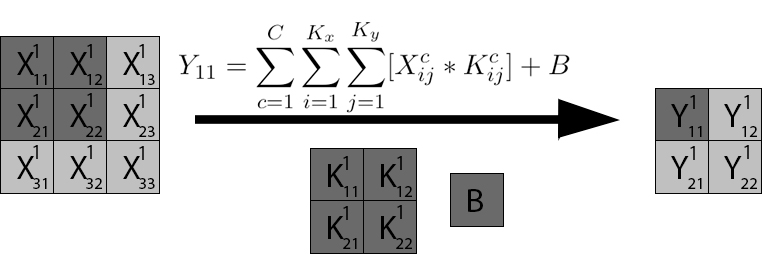
\includegraphics[width=0.8\linewidth]{imagenes/conv_ejemplo_backprop_1.jpg} 
	\caption{Ejemplo de propagación hacia delante en una capa convolucional}
	\label{fig:ejemplo_forward_prop_convolucional}
\end{figure}

La figura \ref{fig:ejemplo_forward_prop_convolucional} ilustra el cálculo de $Y^1_{11}$ para un ejemplo de propagación hacia delante concreto. En dicha figura, \textit{C} representa el número de canales de profundidad del volumen de entrada \textit{X}, mientras que ${K_x}$ y ${K_y}$ se refieren al número de filas y columnas del kernel \textit{K} utilizado, respectivamente. \\
Siguiendo la notación empleada en secciones anteriores, se denotará por $A^c_{ij}$ al valor de $X^c_{ij}$ antes de aplicar la función de activación correspondiente, y por $Z^c_{ij}$ al valor resultante después de aplicar dicha función. Para obtener más detalles, se recomienda consultar el apéndice \ref{backprop_conv_apendice}.

\subsubsection{Sumatoria de gradientes}

\begin{gather}
	\frac{\partial E}{\partial K^c_{11}} = \sum_{i=1}^{I}\sum_{j=1}^{J}  [\frac{\partial E}{\partial Y^c_{ij}} \frac{\partial Y^c_{ij}}{\partial K^c_{11}}] \notag \\
	\frac{\partial E}{\partial X^c_{11}} = \sum_{i=1}^{I}\sum_{j=1}^{J}  [\frac{\partial E}{\partial Y^c_{ij}} \frac{\partial Y^c_{ij}}{\partial Z^c_{11}} \frac{\partial Z^c_{ij}}{\partial A^c_{11}}] \notag 
\end{gather}

Para calcular el gradiente de la función de error con respecto a cada peso ${K_{xy}}$ o entrada ${X_{xy}}$, se debe realizar una sumatoria del gradiente correspondiente sobre cada valor de salida producido por la convolución. En el caso de los pesos asociados a un canal de profundidad $c \in C$, cada peso ${K_{xy}}$ se empleó en el cálculo de cada valor $Y^c_{ij}$. Por otro lado, los valores de la entrada ${X_{xy}}$ contribuyen al cálculo de varios valores de salida $\{Y_1, Y_2\} \in Y$. Este proceso fue detallado anteriormente en la sección \ref{intro_CNN}, y se aborda con mayor profundidad en el apéndice \ref{backprop_conv_apendice}.

\subsubsection{Gradiente de $Y^c_{11}$}

\begin{gather}
	Y^c_{11} = Z^c_{11} K^c_{11} + Z^c_{12} K^c_{12} + Z^c_{21} K^c_{21} + Z^c_{22} K^c_{22} \label{grad_y11_k_11} \\
	\frac{\partial Y^c_{11}}{\partial K^c_{xy}} = \frac{\partial (Z^c_{11} K^c_{11} + Z^c_{12} K^c_{12} + Z^c_{21} K^c_{21} + Z^c_{22} K^c_{22})}{\partial K^c_{xy}} \label{grad_y11_k_12} \\
	\frac{\partial Y^c_{11}}{\partial K^c_{11}} = Z^c_{11}, \hspace{10mm} \frac{\partial Y^c_{11}}{\partial K^c_{12}} = Z^c_{12} \label{grad_y11_k_21}\\
	\frac{\partial Y^c_{11}}{\partial K^c_{21}} = Z^c_{21}, \hspace{10mm} \frac{\partial Y^c_{11}}{\partial K^c_{22}} = Z^c_{22} \label{grad_y11_k_22}
\end{gather}

\begin{gather}
	\frac{\partial Y^c_{11}}{\partial Z^c_{11}} = K^c_{11}, \hspace{10mm} \frac{\partial Y^c_{11}}{\partial Z^c_{12}} = K^c_{12}, \hspace{10mm} \frac{\partial Y^c_{11}}{\partial Z^c_{13}} = 0 \label{grad_y11_z_1} \\
	\frac{\partial Y^c_{11}}{\partial Z^c_{21}} = K^c_{21}, \hspace{10mm} \frac{\partial Y^c_{11}}{\partial Z^c_{22}} = K^c_{22}, \hspace{10mm} \frac{\partial Y^c_{11}}{\partial Z^c_{23}} = 0 \label{grad_y11_z_2} \\
	\frac{\partial Y^c_{11}}{\partial Z^c_{31}} = 0, \hspace{15mm} \frac{\partial Y^c_{11}}{\partial Z^c_{32}} = 0, \hspace{15mm} \frac{\partial Y^c_{11}}{\partial Z^c_{33}} = 0 \label{grad_y11_z_3}
\end{gather}

La fórmula \ref{grad_y11_k_11}, presenta una descomposición de $Y^c_{11}$ en términos de $Z$ y $K$. Esto, es esencial para el cálculo del gradiente, tanto con respecto a Z, (como se detalla en las fórmulas \ref{grad_y11_z_1}, \ref{grad_y11_z_2}, \ref{grad_y11_z_3}), como con respecto a K, (como se muestra en las fórmulas \ref{grad_y11_k_12}, \ref{grad_y11_k_21}, \ref{grad_y11_k_22}). Esta descomposición, permite calcular el gradiente de $Y^c_{11}$ con respecto a cada parámetro de la capa convolucional. \\
Cabe destacar que, para calcular el gradiente con respecto a cada valor del volumen de entrada (X), también debe calcularse la derivada de la función de activación asociada a dicha capa. Es decir, $\frac{\partial Z}{\partial A}$. Sin embargo, dado que este proceso ha sido abordado en secciones anteriores, se omitirá en esta ocasión, al igual que el cálculo del gradiente con respecto al sesgo de cada capa. El propósito de esta omisión es evitar cálculos redundantes y concentrar la atención en los aspectos más relevantes e innovadores. No obstante, es importante señalar que todos los cálculos discutidos en esta documentación, y más, están implementados en el código correspondiente, lo que garantiza que este conocimiento se ha aplicado y verificado en la práctica. \\
Además, dado que todo ha sido realizado manualmente por la misma persona, la mayoría de las variables e índices utilizados en la documentación coinciden perfectamente o son muy similares a los empleados en el código. Esto asegura que cualquier lector con conocimientos básicos de programación pueda comprender gran parte de las implementaciones desarrolladas en este proyecto.

\subsubsection{Gradiente con respecto a los pesos como convolución}

Finalmente, se procede al cálculo de la suma total de gradientes con respecto a cada peso de la capa, conforme a las fórmulas \ref{grad_Y_K_1}, \ref{grad_Y_K_2}, \ref{grad_Y_K_3}, y \ref{grad_Y_K_4}. Para una explicación detallada del cálculo y los fundamentos de cada fórmula, se recomienda consultar el apéndice \ref{backprop_conv_apendice}. Los gradientes resultantes, revelan un patrón claro que refleja la contribución de cada peso en el cálculo del error total.

\begin{gather}
	\frac{\partial E}{\partial K^c_{11}} = \frac{\partial E}{\partial Y^c_{11}} Z^c_{11} + \frac{\partial E}{\partial Y^c_{12}} Z^c_{12} + \frac{\partial E}{\partial Y^c_{21}} Z^c_{21} + \frac{\partial E}{\partial Y^c_{22}} Z^c_{22} \label{grad_Y_K_1} \\
	\frac{\partial E}{\partial K^c_{12}} = \frac{\partial E}{\partial Y^c_{11}} Z^c_{12} + \frac{\partial E}{\partial Y^c_{12}} Z^c_{13} + \frac{\partial E}{\partial Y^c_{21}} Z^c_{22} + \frac{\partial E}{\partial Y^c_{22}} Z^c_{23} \label{grad_Y_K_2} \\	
	\frac{\partial E}{\partial K^c_{21}} = \frac{\partial E}{\partial Y^c_{11}} Z^c_{21} + \frac{\partial E}{\partial Y^c_{12}} Z^c_{22} + \frac{\partial E}{\partial Y^c_{31}} Z^c_{21} + \frac{\partial E}{\partial Y^c_{22}} Z^c_{32} \label{grad_Y_K_3} \\
	\frac{\partial E}{\partial K^c_{22}} = \frac{\partial E}{\partial Y^c_{11}} Z^c_{22} + \frac{\partial E}{\partial Y^c_{12}} Z^c_{23} + \frac{\partial E}{\partial Y^c_{31}} Z^c_{32} + \frac{\partial E}{\partial Y^c_{22}} Z^c_{33} \label{grad_Y_K_4}
\end{gather}

Como se observa en los cálculos realizados, estos coinciden con una operación de convolución entre la entrada \textit{X} y el gradiente respecto a la capa de salida \textit{Y}. Este procedimiento se detalla en la Figura \ref{fig:conv_backprop_como_convolucion_X_Y} \cite{conv_backprop}.

\begin{figure}[H]
	\centering
	\begin{subfigure}{.5\textwidth}
		\hspace{-25mm}
		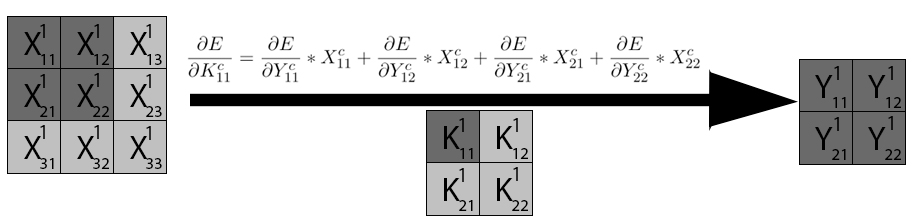
\includegraphics[width=1.4\linewidth]{imagenes/conv_backprop_1.jpg}  
		\caption{Cálculo de $\frac{\partial E}{\partial K^1_{11}}$}
	\end{subfigure}%
	\begin{subfigure}{.5\textwidth}
		\hspace{5mm}
		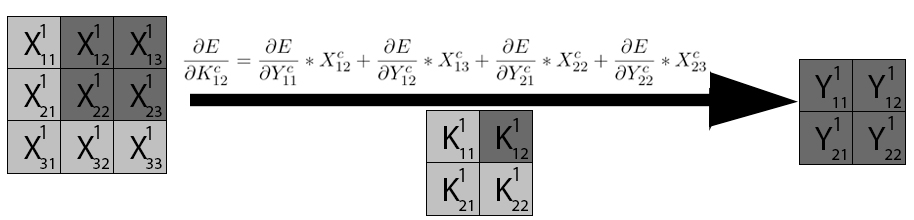
\includegraphics[width=1.4\linewidth]{imagenes/conv_backprop_2.jpg}  
		\caption{Cálculo de $\frac{\partial E}{\partial K^1_{12}}$}
	\end{subfigure}
	\vspace{5mm}
	\begin{subfigure}{.5\textwidth}
		\hspace{-25mm}
		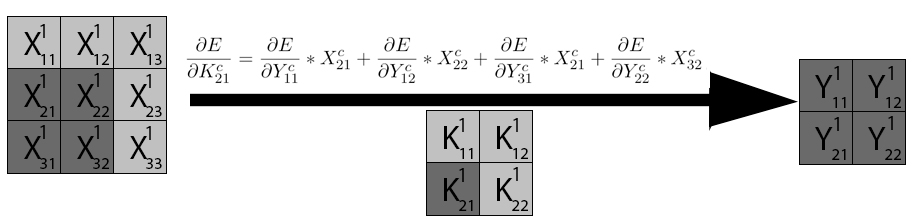
\includegraphics[width=1.4\linewidth]{imagenes/conv_backprop_3.jpg}  
		\caption{Cálculo de $\frac{\partial E}{\partial K^1_{21}}$}
	\end{subfigure}%
	\begin{subfigure}{.5\textwidth}
		\hspace{5mm}
		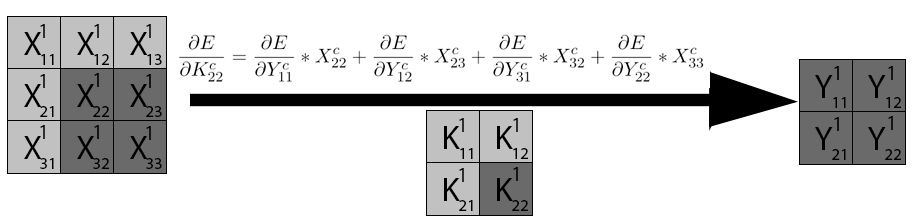
\includegraphics[width=1.4\linewidth]{imagenes/conv_backprop_4.jpg}  
		\caption{Cálculo de $\frac{\partial E}{\partial K^1_{22}}$}
	\end{subfigure}
	\caption{Cálculo del gradiente de la pérdida con respecto a cada filtro como convolución entre la entrada X y la salida Y}
	\label{fig:conv_backprop_como_convolucion_X_Y}
\end{figure}

En la figura \ref{fig:conv_backprop_como_convolucion_X_Y}, cada subfigura $\{(a), (b), (c), (d)\}$ representa el cálculo del gradiente con respecto a un peso específico. Aunque la representación puede parecer algo diferente a simple vista, los cálculos son esencialmente los mismos que los obtenidos anteriormente, con la única diferencia en la forma en que se visualizan.

\subsubsection{Gradiente con respecto a la entrada como convolución}

Por razones de simplicidad, y en consonancia con las recomendaciones de expertos, y la experiencia personal, se empleará ReLU como función de activación en las capas convolucionales. Dado que, la derivada de esta función ya ha sido previamente calculada, (véase la fórmula \ref{deriv_relu}), se considerará esta información para los cálculos subsiguientes.


\begin{gather}
	\frac{\partial E}{\partial A^c_{11}} = \frac{\partial E}{\partial Y^c_{11}} K^c_{11} ReLU'(A^c_{11}) \notag \\
	\frac{\partial E}{\partial A^c_{12}} = (\frac{\partial E}{\partial Y^c_{11}} K^c_{12} + \frac{\partial E}{\partial Y^c_{12}} K^c_{11}) ReLU'(A^c_{12}) \notag \\
	\frac{\partial E}{\partial A^c_{13}} = \frac{\partial E}{\partial Y^c_{12}} K^c_{12} ReLU'(A^c_{13}) \notag \\
	\frac{\partial E}{\partial A^c_{21}} = (\frac{\partial E}{\partial Y^c_{11}} K^c_{21} + \frac{\partial E}{\partial Y^c_{21}} K^c_{11}) ReLU'(A^c_{21}) \notag \\
	\frac{\partial E}{\partial A^c_{22}} = (\frac{\partial E}{\partial Y^c_{11}} K^c_{22} + \frac{\partial E}{\partial Y^c_{12}} K^c_{21} + \frac{\partial E}{\partial Y^c_{21}} K^c_{12} + \frac{\partial E}{\partial Y^c_{22}} K^c_{11}) ReLU'(A^c_{22}) \notag \\
	\frac{\partial E}{\partial A^c_{23}} = (\frac{\partial E}{\partial Y^c_{12}} K^c_{22} + \frac{\partial E}{\partial Y^c_{22}} K^c_{12}) ReLU'(A^c_{22})\notag \\
	\frac{\partial E}{\partial A^c_{31}} = \frac{\partial E}{\partial Y^c_{21}} K^c_{21} ReLU'(A^c_{31})\notag \\
	\frac{\partial E}{\partial A^c_{32}} = (\frac{\partial E}{\partial Y^c_{21}} K^c_{22} + \frac{\partial E}{\partial Y^c_{22}} K^c_{21}) ReLU'(A^c_{32}) \notag \\
	\frac{\partial E}{\partial A^c_{33}} = \frac{\partial E}{\partial Y^c_{22}} K^c_{22} ReLU'(A^c_{33}) \notag
\end{gather}

Tal y como se observa en los cálculos obtenidos, estos corresponden a una convolución completa entre el gradiente con respecto a la capa de salida (Y) y los pesos (K), invertidos tanto horizontal como verticalmente. El proceso de cálculo del gradiente con respecto a cada valor de entrada $x \in X$ se presenta en detalle en la figura \ref{fig:conv_backprop_como_convolucion_Y_W}, mientras que la manera de invertir los pesos se ilustra en la figura \ref{fig:flip_W} \cite{conv_backprop}.

\begin{figure}[H]
	\centering
	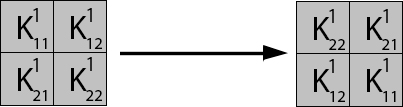
\includegraphics[width=0.8\linewidth]{imagenes/flip_pesos.jpg}  
	\caption{Inversión de los pesos en K tanto horizontal como verticalmente}
	\label{fig:flip_W}
\end{figure}

\begin{figure}[H]
	\centering
	\begin{subfigure}{.5\textwidth}
		\hspace{-25mm}
		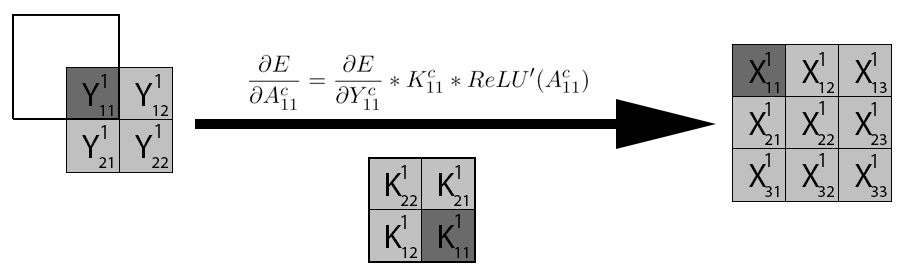
\includegraphics[width=1.4\linewidth]{imagenes/conv_back_entrada_1.jpg}  
		\caption{Gradiente con respecto a $X^1_{11}$}
	\end{subfigure}%
	\begin{subfigure}{.5\textwidth}
		\hspace{5mm}
		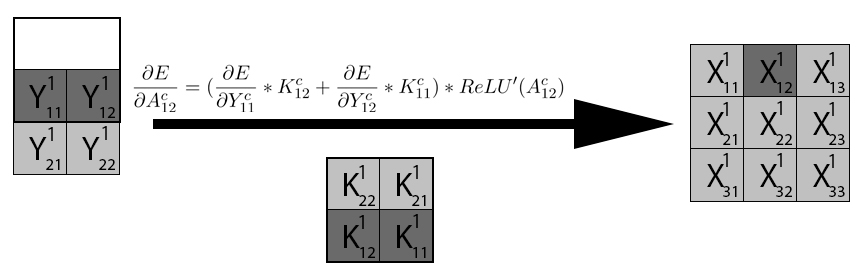
\includegraphics[width=1.4\linewidth]{imagenes/conv_back_entrada_2.jpg}  
		\caption{Gradiente con respecto a $X^1_{12}$}
	\end{subfigure}
	\vspace{5mm}
	\begin{subfigure}{.5\textwidth}
		\hspace{-25mm}
		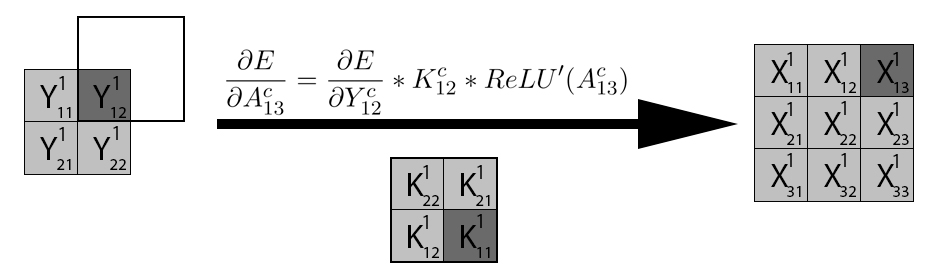
\includegraphics[width=1.4\linewidth]{imagenes/conv_back_entrada_3.jpg}  
		\caption{Gradiente con respecto a $X^1_{13}$}
	\end{subfigure}%
	\begin{subfigure}{.5\textwidth}
		\hspace{5mm}
		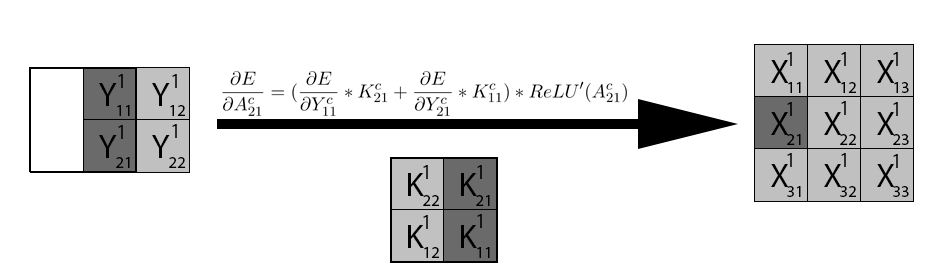
\includegraphics[width=1.4\linewidth]{imagenes/conv_back_entrada_4.jpg}  
		\caption{Gradiente con respecto a $X^1_{21}$}
	\end{subfigure}
	\vspace{5mm}
	\begin{subfigure}{.5\textwidth}
		\hspace{-25mm}
		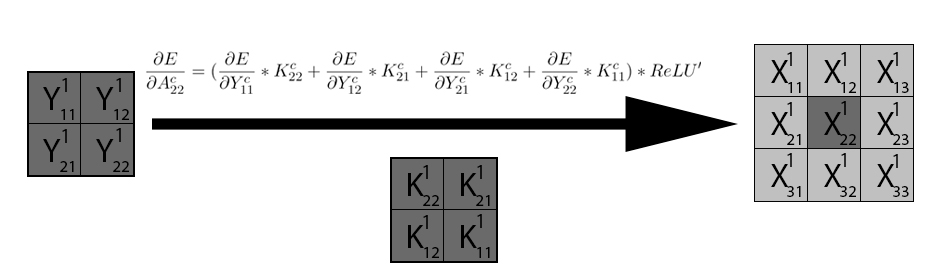
\includegraphics[width=1.4\linewidth]{imagenes/conv_back_entrada_5.jpg}  
		\caption{Gradiente con respecto a $X^1_{22}$}
	\end{subfigure}%
	\begin{subfigure}{.5\textwidth}
		\hspace{5mm}
		\includegraphics[width=1.4\linewidth]{imagenes/conv_back_entrada_6.jpg}  
		\caption{Gradiente con respecto a $X^1_{23}$}
	\end{subfigure}
	\vspace{5mm}
	\begin{subfigure}{.5\textwidth}
		\hspace{-25mm}
		\includegraphics[width=1.4\linewidth]{imagenes/conv_back_entrada_7.jpg}  
		\caption{Gradiente con respecto a $X^1_{31}$}
	\end{subfigure}%
	\begin{subfigure}{.5\textwidth}
		\hspace{5mm}
		\includegraphics[width=1.4\linewidth]{imagenes/conv_back_entrada_8.jpg}  
		\caption{Gradiente con respecto a $X^1_{32}$}
	\end{subfigure}
	\vspace{5mm}
	\begin{subfigure}{.5\textwidth}
		\hspace{-25mm}
		\includegraphics[width=1.4\linewidth]{imagenes/conv_back_entrada_9.jpg}  
		\caption{Gradiente con respecto a $X^1_{33}$}
	\end{subfigure}
	\caption{Cálculo del gradiente de la pérdida con respecto a cada valor de entrada como convolución entre los pesos K y la salida Y}
	\label{fig:conv_backprop_como_convolucion_Y_W}
\end{figure}

Una vez más, los cálculos presentados en la Figura \ref{fig:conv_backprop_como_convolucion_Y_W} coinciden perfectamente con los obtenidos anteriormente, ya que son idénticos. La única diferencia radica en la manera de presentación, la cual ha sido adaptada para ofrecer una mejor comprensión y generalización del proceso. Esta adaptación facilita la automatización de los cálculos y permite una implementación más eficiente en el código.


\subsection{Retropropagación en capas convolucionales con relleno}

Para realizar la retropropagación en una capa convolucional sin relleno, con respecto a la entrada, se emplea una convolución completa. En contraste, para la retropropagación en una capa convolucional con relleno, con respecto a la entrada, se utiliza una convolución sin relleno. Ambos tipos de convoluciones, así como el cálculo detallado de la retropropagación en cada caso, se examinan exhaustivamente en el apéndice \ref{backprop_conv_apendice}.

\begin{figure}[H]
	\centering
	\begin{subfigure}{.5\textwidth}
		\includegraphics[width=1.4\linewidth]{imagenes/full_vs_normal_conv_1.jpg}  
		\caption{Retropropagación con un nivel de relleno}
	\end{subfigure}
	
	\vspace{5mm}
	\begin{subfigure}{.5\textwidth}
		\includegraphics[width=1.4\linewidth]{imagenes/full_vs_normal_conv_2.jpg}  
		\caption{Retropropagación con dos niveles de relleno}
	\end{subfigure}
	\caption{Cálculo del gradiente de la pérdida con respecto a la entrada X con uno y dos niveles de relleno}
	\label{fig:conv_full_vs_normal}
\end{figure}

La razón detrás de esta diferencia se detalla en la figura \ref{fig:conv_full_vs_normal}. En el caso de una convolución con relleno completo, los gradientes se calculan comenzando desde la esquina superior izquierda de la entrada X. Sin embargo, dado que dicha entrada X incluye relleno, no es necesario calcular los gradientes en las posiciones de relleno, ya que estos valores no influyen en los cálculos posteriores.



\subsection{Capa de agrupación máxima}

\subsubsection{Componentes}

\begin{figure}[H]
	\centering
	\includegraphics[scale=0.35]{imagenes/pool_nombres.jpg}  
	\caption{Componentes en una capa de agrupación máxima}
\end{figure}

Al igual que las capas convolucionales, las capas de agupación máxima también presentan una ``ventana'' que se irá deslizando por el volumen de entrada. Sin embargo, el resultado en cada iteración viene dado por el valor máximo contenido en ella. Por tanto, no presenta parámetros asociados.

\subsubsection{Propagación hacia delante}

\begin{figure}[H]
	\centering
	\begin{subfigure}{.5\textwidth}
		\hspace{-10mm}
		\includegraphics[width=1.2\linewidth]{imagenes/maxpool_1.jpg}  
		\caption{Cálculo $Y_{11}$}
	\end{subfigure}%
	\begin{subfigure}{.5\textwidth}
		\hspace{10mm}
		\includegraphics[width=1.2\linewidth]{imagenes/maxpool_2.jpg}  
		\caption{Cálculo $Y_{12}$}
	\end{subfigure}
	
	\vspace{5mm}
	\begin{subfigure}{.5\textwidth}
		\hspace{-10mm}
		\includegraphics[width=1.2\linewidth]{imagenes/maxpool_3.jpg}  
		\caption{Cálculo $Y_{21}$}
	\end{subfigure}%
	\begin{subfigure}{.5\textwidth}
		\hspace{10mm}
		\includegraphics[width=1.2\linewidth]{imagenes/maxpool_4.jpg}  
		\caption{Cálculo $Y_{22}$}
	\end{subfigure}
	\caption{Propagación hacia delante en una capa de agrupación máxima}
	\label{fig:forward_prop_maxpool}
\end{figure}

A diferencia de las capas convolucionales, las capas de agrupación máxima no comparten regiones del volumen de entrada entre distintas iteraciones. Este diferente comportamimento se puede comprobar en la figura \ref{fig:forward_prop_maxpool} con lo que se describe en la figura \ref{fig:forward_prop_convolucional}.


\subsubsection{Propagación hacia delante de X con varios canales de profundidad}

\begin{figure}[H]
	\centering
	\begin{subfigure}{.5\textwidth}
		\hspace{-10mm}
		\includegraphics[width=1.2\linewidth]{imagenes/maxpool_2capas_1.jpg}  
		\caption{Cálculo $Y_{11}$}
	\end{subfigure}%
	\begin{subfigure}{.5\textwidth}
		\hspace{10mm}
		\includegraphics[width=1.2\linewidth]{imagenes/maxpool_2capas_2.jpg}  
		\caption{Cálculo $Y_{12}$}
	\end{subfigure}
	
	\caption{Propagación hacia delante en una capa de agrupación máxima}
	\label{fig:forward_prop_maxpool_canales_profundidad}
\end{figure}

Tal y como se muestra en la figura \ref{fig:forward_prop_maxpool_canales_profundidad}, cada ``ventana'' se desliza sobre el volumen de entrada en un canal de profundidad distinto. Por tanto, al igual que en capas convolucionales, si el volumen de entrada X cuenta con C canales de profundidad, la ventana asociada a la capa de agrupación máxima también contará con C canales de profundidad y cada ventana solo afectará a X en su respectivo canal. Es decir, para la subventana del canal de profundidad $c \in C$, esta solo trabajará sobre la imagen 2D de X asociada al canal c.

\subsubsection{Retropropagación en capa de agrupación máxima}

\begin{figure}[H]
	\centering
	\begin{subfigure}{.5\textwidth}
		\hspace{-10mm}
		\includegraphics[width=1.2\linewidth]{imagenes/back_maxpool_1.jpg}  
		\caption{Cálculo $Y_{11}$}
	\end{subfigure}%
	\begin{subfigure}{.5\textwidth}
		\hspace{10mm}
		\includegraphics[width=1.2\linewidth]{imagenes/back_maxpool_2.jpg}  
		\caption{Cálculo $Y_{12}$}
	\end{subfigure}
	
	\begin{subfigure}{.5\textwidth}
		\hspace{-10mm}
		\includegraphics[width=1.2\linewidth]{imagenes/back_maxpool_3.jpg}  
		\caption{Cálculo $Y_{11}$}
	\end{subfigure}%
	\begin{subfigure}{.5\textwidth}
		\hspace{10mm}
		\includegraphics[width=1.2\linewidth]{imagenes/back_maxpool_4.jpg}  
		\caption{Cálculo $Y_{12}$}
	\end{subfigure}%
	\caption{Retropropagación en capa de agrupación máxima}
	\label{fig:back_prop_maxpool}
\end{figure}

En la Figura \ref{fig:back_prop_maxpool} se muestra un ejemplo de retropropagación en una capa de agrupación máxima. Para calcular el gradiente respecto a la entrada (X) en una capa i de agrupación máxima, suponemos que ya se conoce el gradiente de la pérdida respecto a la salida ($\frac{\partial E}{\partial Y}$) de dicha capa i (se muestra en detalle su cálculo en secciones posteriores). Por tanto, el volumen Y en este caso contendrá dicho gradiente. \\ 
Tomando el ejemplo de la Figura \ref{fig:back_prop_maxpool} (a), se entiende que cuando se realizó la propagación hacia delante de dicha capa i, $Y^1_{11}$ tomó el valor de $X^1_{11}$, pues fue el máximo de entre todos los valores de la ventana (formada por $X^1_{11}$, $X^1_{12}$, $X^1_{21}$, y $X^1_{22}$). Por tanto, dado que en la propagación hacia delante se obtuvo $Y^1_{11} = X^1_{11}$, tiene sentido que el gradiente de $Y^1_{11}$ respecto a $X^1_{11}$ sea 1, pero 0 respecto al resto de valores de X, pues $X^1_{11}$ fue el único valor en influir sobre $Y^1_{11}$. De este modo, el gradiente de la pérdida respecto a la región de X afectada por la ventana $\{X^1_{11}, X^1_{12}, X^1_{21}, X^1_{2} \}$, se puede calcular como se muestra en las fórmulas \ref{grad_plms_x_1}, \ref{grad_plms_x_2}, \ref{grad_plms_x_3}, y \ref{grad_plms_x_4}:

\begin{gather}
	\frac{\partial E}{\partial X^1_{11}} = \frac{\partial E}{\partial Y} \frac{\partial Y}{\partial X^1_{11}} = \frac{\partial E}{\partial Y} 1 = \frac{\partial E}{\partial Y} \label{grad_plms_x_1} \\
	\frac{\partial E}{\partial X^1_{12}} = \frac{\partial E}{\partial Y} \frac{\partial Y}{\partial X^1_{12}} = \frac{\partial E}{\partial Y} 0 \label{grad_plms_x_2} \\
	\frac{\partial E}{\partial X^1_{21}} = \frac{\partial E}{\partial Y} \frac{\partial Y}{\partial X^1_{21}} = \frac{\partial E}{\partial Y} 0 \label{grad_plms_x_3} \\
	\frac{\partial E}{\partial X^1_{22}} = \frac{\partial E}{\partial Y} \frac{\partial Y}{\partial X^1_{22}} = \frac{\partial E}{\partial Y} 0 \label{grad_plms_x_4}
\end{gather}


 
Como el resultado obtenido en cada iteración solo depende del valor máximo de la ventana, tiene sentido que la derivada de la salida Y respecto a la entrada X sea igual a 1 solo en dicho caso y 0 en el resto \cite{max_pool_backprop} \cite{max_pool_backprop_2}.
\subsection{Capa de aplanado}

La capa de aplanado tiene como objetivo la creación de un ``enlace'' entre las capas de convolución y agrupación máxima, con las capas totalmente conectadas. Esto se debe a que, como se mencionó anteriormente, las capas convolucionales y de agrupación máxima trabajan con volúmenes de datos 3D. Sin embargo, las capas totalmente conectadas trabajan con arrays 1D como entrada. Por tanto, la capa de aplanado se encarga de realizar esta conversión de volumen 3D a array 1D y viceversa. 

\subsubsection{Propagación hacia delante}
\begin{figure}[H]
	\centering
	\begin{subfigure}{.5\textwidth}
		\hspace{-10mm}
		\includegraphics[width=2\linewidth]{imagenes/flatten_1.jpg}  
		\caption{Propagación hacia delante de la capa de aplanado con la primera capa de profundidad}
	\end{subfigure}
	\begin{subfigure}{.5\textwidth}
		\hspace{-10mm}
		\includegraphics[width=2\linewidth]{imagenes/flatten_2.jpg}  
		\caption{Propagación hacia delante de la capa de aplanado con la segunda capa de profundidad}
	\end{subfigure}
	
	\caption{Propagación hacia delante en una capa de aplanado}
	\label{fig:forward_prop_flatten_canales_profundidad}
\end{figure}

En la propagación hacia delante, se parte de un volumen de entrada 3D para, mediante un ``aplanado'', convertirlo en un vector 1D que pueda ser usado como entrada para una capa totalmente conectada, tal y como se muestra en la Figura \ref{fig:forward_prop_flatten_canales_profundidad}. \\
Como solo se modifica la forma en la que se agrupan los datos, no requiere la presencia de parámetros \cite{flatten_forward}.

\subsubsection{Retropropagación}

\begin{figure}[H]
	\centering
	\begin{subfigure}{.5\textwidth}
		\hspace{-30mm}
		\includegraphics[width=2\linewidth]{imagenes/back_flatten_1.jpg}  
		\caption{Retropropagación de la primera capa de profundidad en una capa de aplanado}
	\end{subfigure}
	\begin{subfigure}{.5\textwidth}
		\hspace{-30mm}
		\includegraphics[width=2\linewidth]{imagenes/back_flatten_2.jpg}  
		\caption{Retropropagación de la segunda capa de profundidad en una capa de aplanado}
	\end{subfigure}
	
	\caption{Retropropagación en una capa de aplanado}
	\label{fig:back_prop_flatten_canales_profundidad}
\end{figure}

En la retropropagación de una capa de aplanado, se parte de un array 1D y se convierte en un volumen 3D que pueda ser usado para seguir la retropropagación en capas anteriores convolucionales o de agrupación máxima
\cite{flatten_forward}.

\section{OpenCV}

En secciones anteriores se ha indicado que el desarrollo y la implementación de las redes neuronales convolucionales se realizarán exclusivamente mediante el uso de C++, OpenMP, CUDA y cuDNN. Con el fin de optimizar la asignación de recursos y enfocar los esfuerzos en la comprensión y construcción de estas redes, se ha optado por utilizar OpenCV \cite{opencv} para la tarea específica de lectura de las imágenes de entrada. En consecuencia, OpenCV se empleará para convertir las imágenes de entrada en formato PNG o JPG, en un vector de cuatro dimensiones en C++, siguiendo la estructura NCHW (Número de muestras, Canales de profundidad, Altura y Anchura).

\section{OpenMP}

OpenMP \cite{openmp_intro}, es una interfaz de programación de aplicaciones (API), que proporciona directivas de compilador, y rutinas de biblioteca, facilitando así la programación paralela en sistemas con memoria compartida. Diseñada para lenguajes como C, C++ y FORTRAN, OpenMP permite a los desarrolladores escribir código que se ejecute de manera concurrente en múltiples procesadores, optimizando así el rendimiento de las aplicaciones en entornos de multiprocesamiento. \cite{openmp_intro}. \\

A continuación se presentan algunas de sus principales directivas \cite{openmp_directivas}:

\begin{enumerate}[label=\textbullet]
	\item \textbf{Para uso compartido de trabajo paralelo}:
	\begin{enumerate}[label=\textbullet]
		\item \textbf{parallel}: Define una región paralela. Es decir, el código que ejecutarán varios subprocesos en paralelo.
		\item \textbf{for}: Permite que el trabajo realizado en un bucle \textbf{for} dentro de una región paralela se divida entre subprocesos.
		\item \textbf{sections}: Identifica las secciones de código que se van a dividir entre todos los subprocesos.
		\item \textbf{single}: Permite especificar que se debe ejecutar una sección de código en un único subproceso, (no necesariamente en el subproceso principal).
	\end{enumerate}
	\item \textbf{Para el subproceso principal y la sincronización}:
	\begin{enumerate}[label=\textbullet]
		\item \textbf{maestra}: Especifica que solo el subproceso principal debe ejecutar una sección del programa.
		\item \textbf{crítica}: Especifica que el código solo se ejecuta en un subproceso cada vez.
		\item \textbf{barrier}: Sincroniza todos los subprocesos de un equipo; todos los subprocesos se pausan en la barrera hasta que todos los subprocesos ejecutan la barrera.
		\item \textbf{atomic}: Especifica una ubicación de memoria que se actualizará atómicamente.
	\end{enumerate}
\end{enumerate}


\section{CUDA}


CUDA (Compute Unified Device Architecture \cite{cuda_forum}), se define como una plataforma de cómputo paralelo de propósito general, y como un modelo de programación. 
CUDA se distingue, principalmente, por su capacidad para aprovechar la potencia computacional de las GPUs de NVIDIA. Esto, permite la resolución eficiente de problemas complejos, y computacionalmente intensivos. 
Al facilitar la programación de GPUs, y permitir la ejecución de tareas en paralelo, logra acelerar significativamente aplicaciones en áreas como la inteligencia artificial, la simulación científica, y el procesamiento de imágenes, aprovechando la capacidad masiva de cómputo de las GPUs. \\

\subsection{Gestión de memoria}

CUDA permite el desarrollo de aplicaciones en entornos de computación heterogéneos, diferenciando entre memoria asociada a CPU, y memoria asociada a GPU, (separadas por un bus PCI-Express). De esta manera, para ejecutar una sección de código en CPU, sus datos asociados deberán encontrarse en la memoria de la CPU, y, para ejecutar código en GPU, sus datos asociados deberán encontrarse en la memoria asociada a la GPU. 

\subsection{Kernels}

CUDA C++ (el empleado en este proyecto) extiende el lenguaje C++ al permitir al programador definir funciones C++ denominadas ``kernels'', que, cuando se invocan, se ejecutan N veces en paralelo mediante N hebras CUDA distintas, a diferencia de las funciones C++ tradicionales que se ejecutan  una sola vez. Cuando se lanza una función kernel desde la CPU, la ejecución se traslada a la GPU. Una vez en la GPU, esta genera un gran número de hebras y cada una de ellas ejecuta las órdenes especificadas en dicho kernel \cite{cuda_kernels}. \\

\subsection{Jerarquía de hebras}

\begin{figure}[H]
	\centering
	\includegraphics[scale=0.5]{imagenes/cuda_grid.jpg}  
	\caption{Jerarquía de hebras en un grid CUDA}
	\label{fig:cuda_grid}
\end{figure}

Las hebras CUDA se organizan en una cuadrícula o grid compuesta por varios bloques de hebras (véase la Figura \ref{fig:cuda_grid}). De esta manera, cada hebra pertenece a un bloque de hebras, y cada bloque de un mismo kernel pertenece a un mismo grid. Todas las hebras de un mismo grid comparten la misma memoria global. A su vez, las hebras de un mismo bloque se pueden sincronizar y compartir memoria a nivel de bloque, siendo esta más escasa pero presentando una latencia considerablemente menor que la memoria global. CUDA organiza los grids y bloques mediante estructuras que pueden ser 1D, 2D o incluso 3D \cite{Professional_CUDA_C}.

\section{cuDNN (Deep Neural Network)}

Es una librería de primitivas acelerada por GPU para redes neuronales profundas. Proporciona implementaciones altamente optimizadas para módulos como la propagación hacia delante y hacia detrás en capas convolucionales, de agrupación máxima, e incluso con funciones de activación como ReLU o sigmoide, entre otras \cite{cuDNN}. \\
Su meta es obtener el mejor rendimiento posible en GPUs de NVIDIA para casos importantes de aprendizaje profundo. Dados sus buenos resultados, se emplea en gran cantidad de frameworks de aprendizaje profundo, siendo algunos de ellos Caffe2 \cite{Caffe2}, Keras \cite{Keras}, MATLAB \cite{Matlab}, Pytorch \cite{Pytorch}, o TensorFlow \cite{Tensorflow}, entre otras \cite{cuDNN_librerias}. \\
Está diseñada para ser utilizada en aplicaciones de aprendizaje profundo que requieran un poder computacional intensivo, permitiendo a desarrolladores e investigadores aprovechar al máximo las prestaciones de las GPUs de NVIDIA. Entre sus puntos fuertes, destacan la compatibilidad con múltiples arquitecturas de  GPU, su optimización de la memoria, y su flexibilidad y facilidad de integración. Por todo esto y más, se ha convertido en un compotente esencial en el desarrollo de soluciones de inteligencia artificial, facilitando la investigación y la innovación en el campo del aprendizaje profundo.


\subsection{Manejador}

cuDNN asume que los datos necesarios se encuentran ya en GPU y accesibles desde device. Se hablará de esto con más detalle en la sección sobre CUDA y GPU. \\
Una aplicación que use cuDNN requiere de la inicialización de un manejador o handle. Dicho manejador será requerido por cuDNN en cada operación que se quiera realizar con dicha librería, permitiendo al usuario un control explícito sobre el funcionamiento de la misma aunque este emplee múltiples hebras o GPUs. \\
Por ejemplo, en el caso de múltiples GPUs, se pueden asociar diferentes dispositivos con diferentes hebras del host, de forma que cada una tenga un manejador de cuDNN distinto. Así, las llamadas a cuDNN con distinto manejador se ejecutarán en una GPU distinta \cite{cuDNN_core_concepts}.

\subsection{Tensores}

En cuDNN, un tensor es un vector multidimensional, empleado para representar datos. Se define a través de parámetros como el número de dimensiones, el tipo de dato (por ejemplo, punto flotante de 32 o 64 bits), el tamaño de cada dimensión, y el paso de cada dimensión (esto es, el incremento necesario para acceder al siguiente elemento en esa dimensión). Esta definición flexible permite configuraciones de datos complejas, incluyendo dimensiones superpuestas y diversas disposiciones de datos. Por lo tanto, las operaciones en cuDNN reciben tensores como entrada y producen tensores como salida \cite{cuDNN_core_concepts}.

\subsubsection{Tensor 3D}
Un tensor 3D se suele emplear para representar un volumen 3D como podría ser una imagen RGB. Sus dimensiones se describen mediante 3 letras: B, M y N.

\begin{enumerate}
	\item \textbf{B}: Tamaño del batch
	\item \textbf{M}: Filas por imagen 2D
	\item \textbf{N}: Columnas por imagen 2D
\end{enumerate}

\subsubsection{Tensor 4D \label{NCHW}}
Suele representar conjuntos de imágenes 2D. Sus dimensiones son N, C, H, W

\begin{enumerate}
	\item \textbf{N}: Tamaño del batch
	\item \textbf{C}: Número de imágenes 2D
	\item \textbf{H}: Filas por imagen 2D
	\item \textbf{W}: Columnas por imagen 2D
\end{enumerate}

cuDNN permite varios formatos pero usaremos el formato de tensores NCHW por compatibilidad con el resto de implementaciones desarrolladas en este proyecto.


\subsubsection{Representación de un tensor 4D}

\begin{figure}[H]
	\centering
	\includegraphics[scale=0.5]{imagenes/ejemplo_tensor.png}  
	\caption{Ejemplo de tensor 4D con dimensiones: N=1, C=1, H=5, y W=6}
	\label{fig:ejemplo_tensor}
\end{figure}

En la figura \ref{fig:ejemplo_tensor} se muestra un conjunto de imágenes 3D con las siguientes dimensiones:
\begin{enumerate}
	\item \textbf{N}: Tamaño del batch, 1
	\item \textbf{C}: Número de imágenes 2D o canales por imagen 3D, 2
	\item \textbf{H}: Filas por imagen 2D, 5
	\item \textbf{W}: Columnas por imagen 2D, 6
\end{enumerate}

\begin{figure}[H]
	\centering
	\includegraphics[scale=0.5]{imagenes/tensor_nchw.png}  
	\caption{Ejemplo de tensor 4D NCHW con dimensiones: N=1, C=1, H=5, y W=6}
	\label{fig:tensor_nchw}
\end{figure}

En la figura \ref{fig:tensor_nchw} se muestra como se almacena en memoria el volumen de datos de la figura \ref{fig:ejemplo_tensor} según el formato NCHW. Esto es, por cada imagen 3D n$\in$\{0,...,N-1\}, almacenar cada canal c$\in$\{0,...,C\} según una ordenación por filas.

\subsection{Principales funciones}

A continuación, se mencionarán las principales funciones de cuDNN que se han empleado en este proyecto, siendo las responsables tanto de la propagación hacia delante como de la retropropagación en capas convolucionales y de agrupación máxima, entre otras.

\subsubsection{cudnnConvolutionForward}

Dado el manejador cuDNN, el tensor de la entrada, el tensor de los pesos, y el algoritmo de convolución especificado, la función cudnnConvolutionForward genera el tensor de salida. Aunque el procedimiento puede variar, los resultados son equivalentes a los descritos en secciones anteriores. En consecuencia, cudnnConvolutionForward realiza la propagación hacia delante en una capa convolucional. Para obtener información adicional, consulte el apéndice \ref{cudnnConvolutionForward} \cite{cuDNN_conv_fwd}.

\subsubsection{cudnnPoolingForward}

Dado el manejador cuDNN y el tensor de la entrada,  la función cudnnPoolingForward genera el tensor de salida para una capa de agrupación máxima. Aunque el procedimiento puede variar, los resultados son equivalentes a los descritos en secciones anteriores. Para obtener información adicional, consulte el apéndice \ref{cudnnPoolingForward} \cite{cuDNN_pool_fwd}.

\subsubsection{cudnnPoolingBackward}

Para una capa \texttt{i} específica, dado el manejador cuDNN, el tensor de la salida, y el tensor de entrada de dicha capa \texttt{i}, la función cudnnPoolingForward genera el tensor de entrada mediante el cálculo de la retroprogapagación a través de la misma. Una vez más, los resultados son equivalentes a los descritos en secciones anteriores. Para obtener información adicional, consulte el apéndice \ref{cudnnPoolingBackward} \cite{cuDNN_pool_fwd}.

\subsubsection{cudnnConvolutionBackwardFilter}

Para una capa \texttt{i} específica, dado el manejador cuDNN, el tensor de entrada, el tensor del gradiente con respecto a la salida, y el algoritmo de convolución especificado, la función cudnnConvolutionBackwardFilter genera el tensor del gradiente con respecto a los pesos, mediante el cálculo de la retroprogapagación a través de la misma. Aunque el procedimiento puede variar, los resultados son equivalentes a los descritos en secciones anteriores. Para obtener información adicional, consulte el apéndice \ref{cudnnConvolutionBackwardFilter} \cite{cuDNN_conv_back_w}.

\subsubsection{cudnnConvolutionBackwardData}
Realiza la retropropagación respecto a los datos de entrada en una capa convolucional.

Para una capa \texttt{i} específica, dado el manejador cuDNN, el tensor del gradiente con respecto a la salida, el tensor de los pesos, y el algoritmo de convolución especificado, la función cudnnConvolutionBackwardFilter genera el tensor del gradiente con respecto a la entrada, mediante el cálculo de la retroprogapagación a través de la misma. Aunque el procedimiento puede variar, los resultados son equivalentes a los descritos en secciones anteriores. Para obtener información adicional, consulte el apéndice \ref{cudnnConvolutionBackwardData} \cite{cuDNN_conv_back_x}.

